\documentclass[12pt]{article}
\usepackage[margin=1in]{geometry}
\usepackage{amsmath}
\usepackage{amsfonts}
\usepackage{amssymb}
\usepackage{amsthm}
\usepackage{graphicx}
\usepackage{tikz}
\usetikzlibrary{arrows}
\usepackage{esvect}
\usepackage{pgfplots}
\usepackage{xcolor}

\title{Math 218-1 Workbook}
\author{Aaron Greicius, Gabriela Laboska}
\date{Last update: 09/21/2026}

\newenvironment{solution}{\begin{proof}[Solution]}{\end{proof}}



\begin{document}
	
	\maketitle
	\vspace{2cm}
	\begin{itemize}
		\item This workbook was made to be a companion to the already existing Math 218-1 textbook. It contains exercises to help you better understand the material and prepare for any upcoming exams/quizzes. Always read the corresponding section of the book before attempting these exercises.
		\item This workbook will be updated regularly, so please make sure to have the latest version at all times.
		\item If you notice any typos or inconsistencies, please email Gabriela Laboska 
		
		(gabriela.laboska@northwestern.edu).
	\end{itemize}
	
	\newpage
	
	\tableofcontents
	\newpage
	
	\section{What is a function?}
	
	\begin{enumerate}
		\item Write the following sets using interval notation and sketch them on the real number line. Your answer should be an interval or a union of intervals.
		\begin{enumerate}
			\item $\{x\in\mathbb{R}| -1\leq x<5\}$
			\item $\{x\in\mathbb{R}| x>2 \text{ or } x<-2\}$
			\item $\{x\in\mathbb{R}| x \text{ is a nonnegative number whose absolute value is less than } 3\}$
		\end{enumerate}
		
		\begin{solution}
			\begin{itemize}
				\item[(a)] 	$[-1,5)$.
				\begin{center}				
					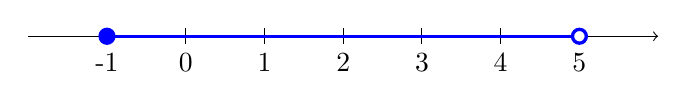
\begin{tikzpicture}
						% Number line
						\draw[->] (-2,0) -- (6,0);
						
						% Tick marks
						\foreach \x in {-1,0,1,2,3,4,5}
						\draw (\x,0.1) -- (\x,-0.1);
						
						% Labels
						\foreach \x in {-1,0,1,2,3,4,5}
						\node[below] at (\x,-0.1) {\x};
						
						% Interval
						\draw[very thick, blue] (-1,0) -- (5,0);
						
						% Closed endpoint at -1
						\draw[very thick, blue, fill=blue] (-1,0) circle (2.5pt);
						
						% Open endpoint at 5
						\draw[very thick, blue, fill=white] (5,0) circle (2.5pt);
					\end{tikzpicture}
				\end{center}
				\item[(b)] 	$(-\infty,-2)\cup (2,\infty)$.
				\begin{center}
					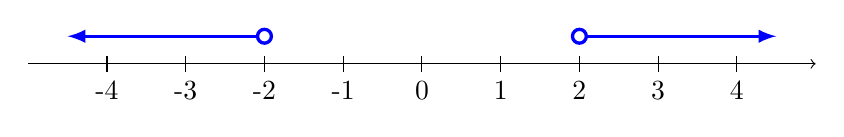
\begin{tikzpicture}
						% Number line
						\draw[->] (-5,0) -- (5,0);
						
						% Tick marks
						\foreach \x in {-4,-3,-2,-1,0,1,2,3,4}
						\draw (\x,0.1) -- (\x,-0.1);
						
						% Labels
						\foreach \x in {-4,-3,-2,-1,0,1,2,3,4}
						\node[below] at (\x,-0.1) {\x};
						
						% Blue interval
						\draw[very thick, blue, -latex] (-2,0.35) -- (-4.5,0.35);
						\draw[very thick, blue, -latex] (2,0.35) -- (4.5,0.35);
						
						% Hollow endpoints
						\draw[very thick, blue, fill=white] (-2,0.35) circle (2.5pt);
						\draw[very thick, blue, fill=white] (2,0.35) circle (2.5pt);
					\end{tikzpicture}
				\end{center}
				\item[(c)] $[0,3)$.
				\begin{center}
					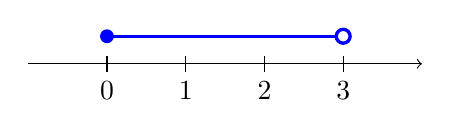
\begin{tikzpicture}
						% Number line
						\draw[->] (-1,0) -- (4,0);
						
						% Tick marks
						\foreach \x in {0,1,2,3}
						\draw (\x,0.1) -- (\x,-0.1);
						
						% Labels
						\foreach \x in {0,1,2,3}
						\node[below] at (\x,-0.1) {\x};
						
						% Blue interval
						\draw[very thick, blue] (0,0.35) -- (3,0.35);
						
						% Closed endpoint at 0
						\fill[blue] (0,0.35) circle (2.5pt);
						
						% Open endpoint at 3
						\draw[very thick, blue, fill=white] (3,0.35) circle (2.5pt);
					\end{tikzpicture}
				\end{center}
			\end{itemize}
		\end{solution}
		\item Consider the graphs given below. Determine which of them are graphs of functions.

		\begin{enumerate}
			\item 
			
		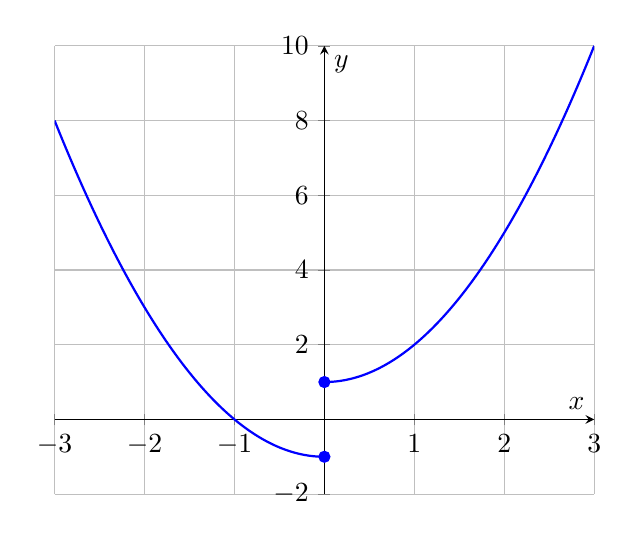
\begin{tikzpicture}
			\begin{axis}[
				axis lines = middle,
				xlabel = {$x$},
				ylabel = {$y$},
				xmin = -3, xmax = 3,
				ymin = -2, ymax = 10,
				grid = both
				]
				
				% f(x) = x^2 - 1 for x <= 0
				\addplot[
				domain=-3:0,
				samples=100,
				blue,
				thick
				] {x^2 - 1};
				
				% f(x) = x^2 + 1 for x >= 0
				\addplot[
				domain=0:3,
				samples=100,
				blue,
				thick
				] {x^2 + 1};
				
				\addplot[
				only marks,
				mark=*,
				mark size=2pt,
				blue
				] coordinates {(0,-1)};
				
				\addplot[
				only marks,
				mark=*,
				mark size=2pt,
				blue
				] coordinates {(0,1)};
				
				
			\end{axis}
			
		
		\end{tikzpicture}
		
		\item 
		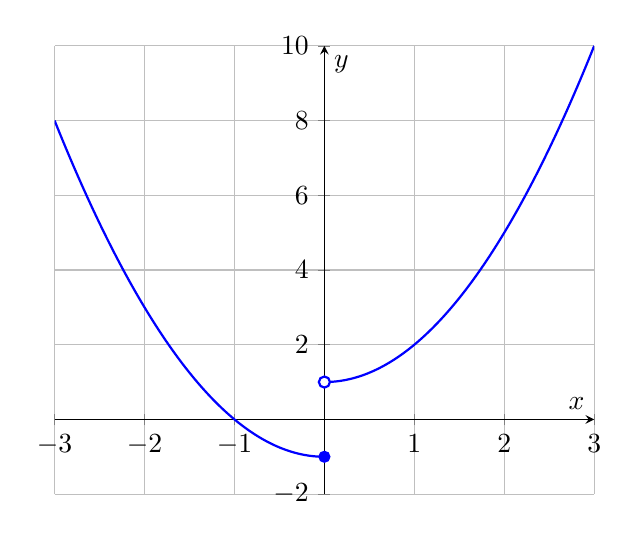
\begin{tikzpicture}
			\begin{axis}[
				axis lines = middle,
				xlabel = {$x$},
				ylabel = {$y$},
				xmin = -3, xmax = 3,
				ymin = -2, ymax = 10,
				grid = both
				]
				
				% f(x) = x^2 - 1 for x <= 0
				\addplot[
				domain=-3:0,
				samples=100,
				blue,
				thick
				] {x^2 - 1};
				
				% f(x) = x^2 + 1 for x >= 0
				\addplot[
				domain=0:3,
				samples=100,
				blue,
				thick
				] {x^2 + 1};
				
				\addplot[
				only marks,
				mark=*,
				mark size=2pt,
				blue
				] coordinates {(0,-1)};
				
				\addplot[
				only marks,
				mark=*,
				mark size=2pt,
				fill=white,
				draw=blue,
				thick
				] coordinates {(0,1)};
				
			\end{axis}
			
			
		\end{tikzpicture}
		
		\item
	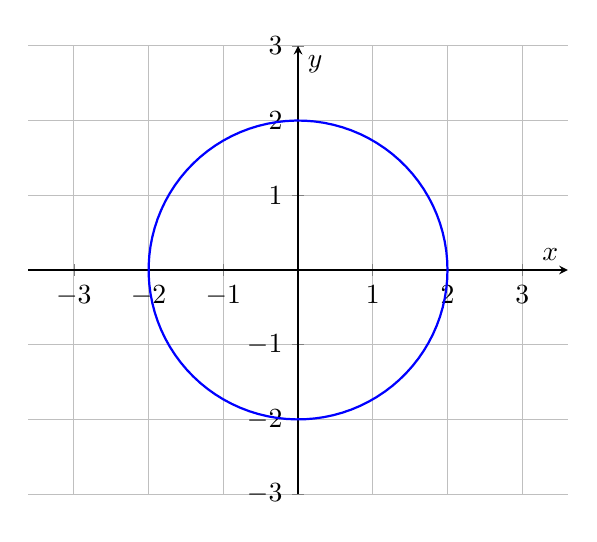
\begin{tikzpicture}
		\begin{axis}[
			axis lines = middle,
			xlabel = {$x$},
			ylabel = {$y$},
			xmin = -3, xmax = 3,
			ymin = -3, ymax = 3,
			xtick={-3,-2,-1,0,1,2,3},
			ytick={-3,-2,-1,0,1,2,3},
			grid = both,
			axis equal
			]
			
			% Circle x^2 + y^2 = 4
			\addplot[
			domain=0:360,
			samples=100,
			blue,
			thick
			] ({2*cos(x)}, {2*sin(x)});
			
		\end{axis}
	\end{tikzpicture}

	\item 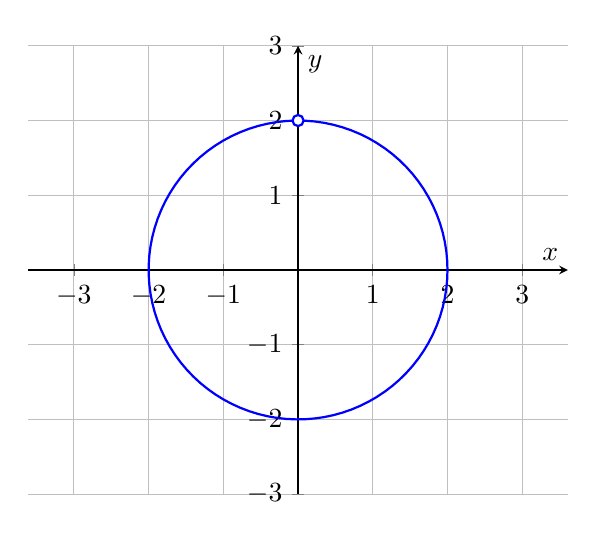
\begin{tikzpicture}
		\begin{axis}[
			axis lines = middle,
			xlabel = {$x$},
			ylabel = {$y$},
			xmin = -3, xmax = 3,
			ymin = -3, ymax = 3,
			xtick={-3,-2,-1,0,1,2,3},
			ytick={-3,-2,-1,0,1,2,3},
			grid = both,
			axis equal
			]
			
			% Circle x^2 + y^2 = 4
			\addplot[
			domain=0:360,
			samples=100,
			blue,
			thick
			] ({2*cos(x)}, {2*sin(x)});
			
			% Hole at (2,0)
			\addplot[
			only marks,
			mark=*,
			mark size=2pt,
			fill=white,
			draw=blue,
			thick
			] coordinates {(0,2)};
			
		\end{axis}
	\end{tikzpicture}
	\end{enumerate}
	
	\begin{solution}
		\begin{itemize}
			\item[(a)] 	Not a function. The $y$-axis is a vertical line that intersects the graph at 2 points. Therefore, the graph fails the vertical line test.
			\item[(b)] 	This is a graph of a function. Every vertical line intersects the graph at at most one point.
			\item[(c)] Not a function. The $y$-axis is a vertical line that intersects the graph at two points. Therefore, the graph fails the vertical line test.
			\item[(d)] While the $y$-axis intersects the graph at only one point, the vertical line $x=1$ intersects it at two points. Therefore, this is not the graph of a function.
		\end{itemize}
	\end{solution}

	
		\item The graphs of some functions are given below. Assume that the functions are defined only on the given grid.
		\begin{itemize}
			\item Find the domain and range of the functions based on the graphs. Your answer should be an interval or a union of intervals.
			\item For each function, find the values of $f(0), f(1), f(-1)$, or state that a value does not exist.
			\item For each function, find all the values of $x$ such that $f(x)=0$ (if any).
		\end{itemize}
		\begin{enumerate}
			\item 
			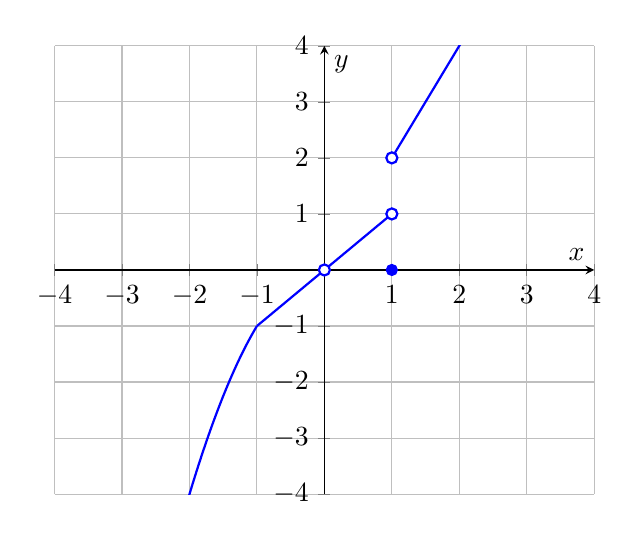
\begin{tikzpicture}
				\begin{axis}[
					axis lines = middle,
					xlabel = {$x$},
					ylabel = {$y$},
					xmin = -4, xmax = 4,
					ymin = -4, ymax = 4,
					xtick={-4,-3,-2,-1,0,1,2,3,4},
					ytick={-4,-3,-2,-1,0,1,2,3,4},
					grid = both
					]
					
					% Concave down quadratic on (-infty,-1)
					\addplot[
					domain=-3:-1,
					samples=100,
					blue,
					thick
					] {-x^2};
					
					% Linear function on (-1,1)
					\addplot[
					domain=-1:1,
					samples=100,
					blue,
					thick
					] {x};
					
					% Concave up quadratic y = x^2 + 1 on (1,infty)
					\addplot[
					domain=1:3,
					samples=100,
					blue,
					thick
					] {2*x};
					
					% Hole at (1,2)
					\addplot[
					only marks,
					mark=*,
					mark size=2pt,
					fill=white,
					draw=blue,
					thick
					] coordinates {(1,2)};
					
					% Hole at (1,1)
					\addplot[
					only marks,
					mark=*,
					mark size=2pt,
					fill=white,
					draw=blue,
					thick
					] coordinates {(1,1)};
					
						% Hole at (0,0)
					\addplot[
					only marks,
					mark=*,
					mark size=2pt,
					fill=white,
					draw=blue,
					thick
					] coordinates {(0,0)};
					
					% Point at (1,0)
					\addplot[
					only marks,
					mark=*,
					mark size=2pt,
					blue
					] coordinates {(1,0)};
					
				\end{axis}
			\end{tikzpicture}
			
		
			
			\item 
			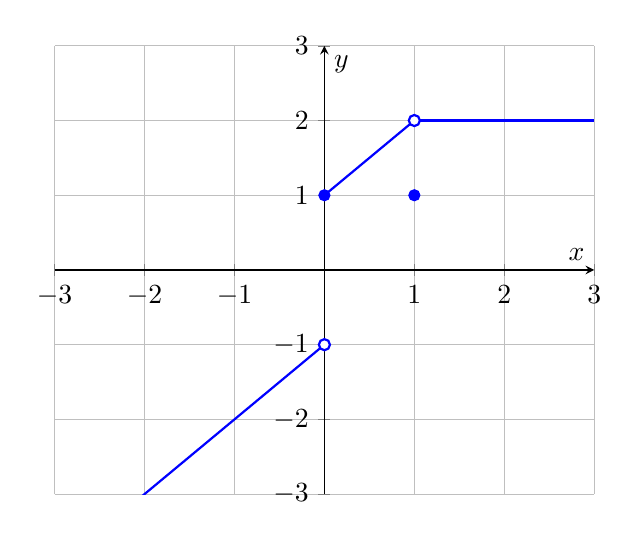
\begin{tikzpicture}
				\begin{axis}[
					axis lines = middle,
					xlabel = {$x$},
					ylabel = {$y$},
					xmin = -3, xmax = 3,
					ymin = -3, ymax = 3,
					xtick={-3,-2,-1,0,1,2,3},
					ytick={-3,-2,-1,0,1,2,3},
					grid = both
					]
					
					% y = x - 1 for x < 0
					\addplot[
					domain=-3:0,
					samples=100,
					blue,
					thick
					] {x - 1};
					
					% y = x + 1 for 0 < x < 1
					\addplot[
					domain=0:1,
					samples=100,
					blue,
					thick
					] {x + 1};
					
					% y = 2 for x > 1
					\addplot[
					domain=1:3,
					samples=100,
					blue,
					thick
					] {2};
					
					% Hole at (0,-1)
					\addplot[
					only marks,
					mark=*,
					mark size=2pt,
					fill=white,
					draw=blue,
					thick
					] coordinates {(0,-1)};
					
					% Point at (0,1)
					\addplot[
					only marks,
					mark=*,
					mark size=2pt,
					blue
					] coordinates {(0,1)};
					
					% Hole at (1,2)
					\addplot[
					only marks,
					mark=*,
					mark size=2pt,
					fill=white,
					draw=blue,
					thick
					] coordinates {(1,2)};
					
					% Point at (1,1)
					\addplot[
					only marks,
					mark=*,
					mark size=2pt,
					blue
					] coordinates {(1,1)};
					
				\end{axis}
			\end{tikzpicture}
					
		\end{enumerate}
		
		\begin{solution}
			\begin{itemize}
				\item[(a)] The domain is $[-2,0)\cup (0,2)$, the range is $[-4,1)\cup(2,4]$. $f(0)$ does not exist, $f(1)=0$ and $f(-1)=-1$. $x=1$ is the only value of $x$ such that $f(x)=0$.
				\item[(b)] The domain is $[-2,3]$ and the range is $[-3,-1)\cup[1,2]$. $f(0)=1,f(1)=1,f(-1)=-2$. There are no $x$ such that $f(x)=0$.
			\end{itemize}
		\end{solution}
		
		\item Determine whether the following statements are true or false. Justify your reasoning.
		\begin{enumerate}
			\item It is not possible for two intervals to intersect at exactly one point.
		
			\item A function assigns exactly one output to each input.
		
			\item The following points are points on the graph of a function $(0,2),(1,1),(1,2),(2,1)$.
			
			\item The following points are points on the graph of a function $(0,2),(1,2),(2,1),(-1,1)$.
		
			\item
				If the range of a function consists of only one point, the domain also consists of only one point.
		
		\end{enumerate}
		
		\begin{solution}
			\begin{itemize}
				\item[(a)] 	False. For example, the intervals $(-1,1]$ and $[1,2]$ intersect at exactly one point.
				\item[(b)] 	True. This is part of the definition of a function.
				\item[(c)] False. The input 1 has two outputs 1 and 2.
				\item[(d)] 	True. Every input has exactly one output (even though two different inputs have the same output).
				\item[(e)] False. It is possible for different inputs of a function to have the same output. An example is the function $f$ with domain $\{1,2\}$ and range $\{3\}$, defined by $f(1)=3,f(2)=3$ (or any other constant function).
			\end{itemize}
		\end{solution}
	\end{enumerate}
	
	\newpage
	\section{Linear and Quadratic Functions}
	
		\begin{enumerate}
			
		\item Determine which of the following functions are linear. For those that are:
		\begin{itemize} 
			\item Find the $x$ and $y$-intercepts (if any).
			\item Determine whether they are increasing or decreasing.
			\item Find the $x$ for which the function is positive/negative.
			\item Find the minimum/maximum (if any).
			\item Sketch the graph of the function.
		\end{itemize}
		\begin{enumerate}
			\item $f(x)=-\dfrac{1}{2}x+2$
		
			\item $f(x)=-\dfrac{1}{2x}+2$
			
			\item $f(x)=(x+2)^2-(x-2)^2$
		
			\item $f(x)=-(x+1)(x-3)+x(x-2)$
			
			\item $f(x)=\dfrac{x^2-1}{x-1}$
		
		\end{enumerate}
		
		
		\begin{solution}
			\begin{itemize}
				\item[(a)] The function is linear. 
				
				To find the $x$-intercept, we need to solve the equation $-\dfrac{1}{2}x+2=0$. Solving the equation, we get $x=4$, so the $x$-intercept is $(4,0)$.
				
				To find the $y$-intercept, set $x=0$. We get $y=2$, so the $y$-intercept is $(0,2)$. 
				
				Since the slope $m=-\dfrac{1}{2}<0$, the function is decreasing on $\mathbb{R}$, and hence, has no minimum/maximum.
				
				To find the $x$ for which the function is positive/negative, we need to solve the inequalities $f(x)>0$ and $f(x)<0$. Note that it is enough to solve one of them.
				$$f(x)>0$$
				$$-\dfrac{1}{2}x+2>0$$
				$$-\dfrac{1}{2}x>-2$$
				$$x<4.$$
				Therefore, the function is positive on $(-\infty,4)$ and negative on $(4,\infty)$.
				
				
				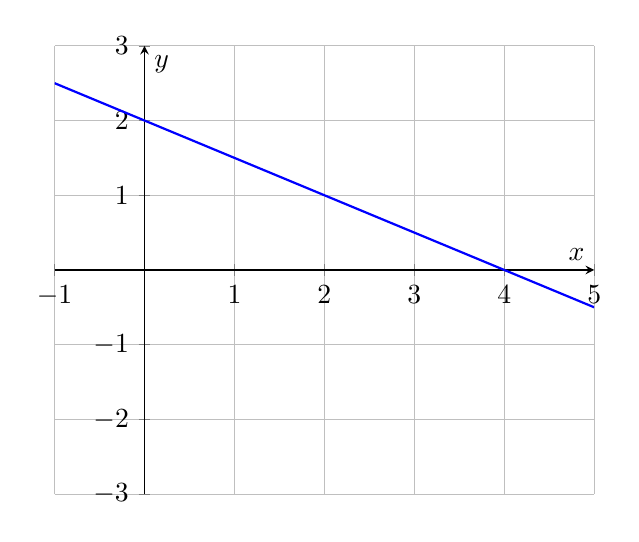
\begin{tikzpicture}
					\begin{axis}[
						axis lines = middle,
						xlabel = {$x$},
						ylabel = {$y$},
						xmin = -1, xmax = 5,
						ymin = -3, ymax = 3,
						xtick={-1,0,1,2,3,4,5},
						ytick={-3,-2,-1,0,1,2,3},
						grid = both
						]
						
						% f(x) = -1/2 x + 2
						\addplot[
						domain=-1:5,
						samples=100,
						blue,
						thick
						] {-0.5*x + 2};
						
					\end{axis}
				\end{tikzpicture}
				
				\item[(b)] Not linear.
				\item[(c)] 	Simplifying, we get $f(x)=(x^2+4x+4)-(x^2-4x+4)=8x$, so the function is linear.
				
				To find the $x$-intercept, we need to solve the equation $8x=0$. Solving the equation, we get $x=0$, so the $x$-intercept is $(0,0)$.
				
				To find the $y$-intercept, set $x=0$. We get $y=0$, so the $y$-intercept is $(0,0)$. 
				
				Since the slope $m=8>0$, the function is increasing, and hence, has no minimum/maximum.
				
				To find the $x$ for which the function is positive/negative, we need to solve the inequalities $f(x)>0$ and $f(x)<0$. Note that it is enough to solve one of them.
				$$f(x)>0$$
				$$8x>0$$
				$$x>0.$$
				
				Therefore, the function is negative on $(-\infty,0)$ and positive on $(0,\infty)$.
				
				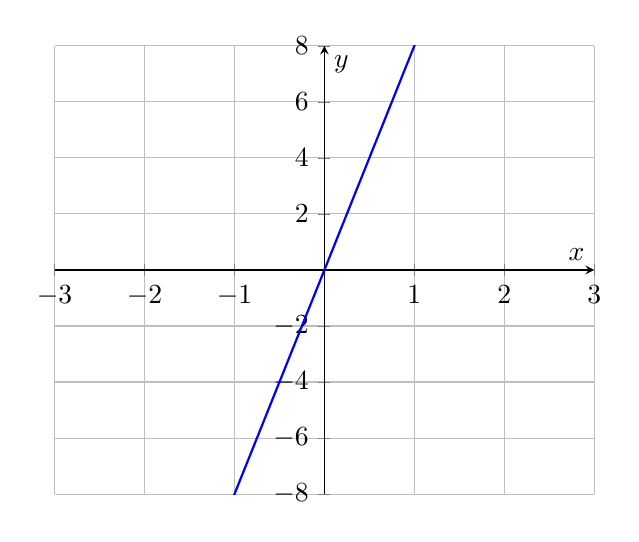
\begin{tikzpicture}
					\begin{axis}[
						axis lines = middle,
						xlabel = {$x$},
						ylabel = {$y$},
						xmin = -3, xmax = 3,
						ymin = -8, ymax = 8,
						xtick={-3,-2,-1,0,1,2,3},
						ytick={-8,-6,-4,-2,0,2,4,6,8},
						grid = both
						]
						
						% f(x) = 8x
						\addplot[
						domain=-3:3,
						samples=100,
						blue,
						thick
						] {8*x};
						
					\end{axis}
				\end{tikzpicture}
				\item[(d)] 
					Simplifying, we get $f(x)=-(x^2-3x+x-3)+(x^2-2x)=-x^2+2x+3+x^2-2x=3$, so the function is constant and, therefore, linear.
					
					There is no $x$-intercept and the $y$-intercept is $(0,3)$. 
					
					Since the function is constant, it is not increasing nor decreasing, and both the minimum and maximum are $3$, achieved at every $x\in\mathbb{R}$.
					
					Since $f(x)=3>0$, the function is positive for all $x\in\mathbb{R}$.
					
					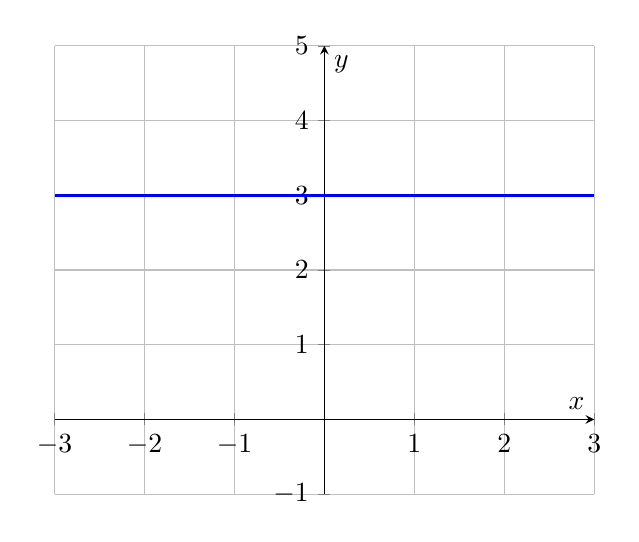
\begin{tikzpicture}
						\begin{axis}[
							axis lines = middle,
							xlabel = {$x$},
							ylabel = {$y$},
							xmin = -3, xmax = 3,
							ymin = -1, ymax = 5,
							xtick={-3,-2,-1,0,1,2,3},
							ytick={-1,0,1,2,3,4,5},
							grid = both
							]
							
							% f(x) = 3
							\addplot[
							domain=-3:3,
							blue,
							very thick
							] {3};
							
						\end{axis}
					\end{tikzpicture}
				\item[(e)]  	Not linear, the domain of this function is $\mathbb{R} \setminus\{1\}$, and the domain of all linear functions is an interval. (Even though when you simplify the expression algebraically, you get $\dfrac{(x-1)(x+1)}{x-1}=x+1$.)
				
			\end{itemize}
			\end{solution}
		
		\item Solve the following equations.
		\begin{enumerate}
			\item $x^2-5x-14=0$
			
			\item $x^2=x$
			
			\item $x^2=3x-5$
			
			\item $x^2-x+(x+\dfrac{1}{2})^2=8\dfrac{1}{4}$
		
			\item $(3x-2)-(x-3)^2=-11$
		
			\item $x+\dfrac{1}{x}=5,\ x\neq 0$
		
			\item $\dfrac{x+1}{x-1}=3-\dfrac{x-2}{x+2},\ x\neq1,x\neq-2$
		
		\end{enumerate}
		
		\begin{solution}
			\begin{itemize}
				\item[(a)] 	Use the quadratic formula.
				$$x_{1/2}=\dfrac{5\pm\sqrt{25+4\cdot 14}}{2}=\dfrac{5\pm\sqrt{81}}{2}=\dfrac{5\pm9}{2}.$$
				Thus, $x_1=\dfrac{5-9}{2}=-2$ and $x_2=\dfrac{5+9}{2}=7$.
				\item[(b)] 	\begin{align*}
					x^2-x&=0\\
					x(x-1)&=0\\
					x=0 \text{ or } &x=1.
				\end{align*}
				\item[(c)] The equation is equivalent to $x^2-3x+5=0$. Since the discriminant is $D=(-3)^2-4\cdot 5=9-20=-11<0$, the equation has no real solutions.
				\item[(d)] 	$$x^2-x+(x+\dfrac{1}{2})^2=8\dfrac{1}{4}$$
				$$x^2-x+x^2+x+\dfrac{1}{4}=8\dfrac{1}{4}$$
				$$2x^2=8$$
				$$x^2=4$$
				$$x_{1/2}=\pm2.$$
				\item[(e)] $$(3x-2)-(x-3)^2=-11$$
				$$3x-2-(x^2-6x+9)=-11$$
				$$3x-2-x^2+6x-9+11=0$$
				$$-x^2+9x=0$$
				$$x(-x+9)=0$$
				$$x=0 \text{ or } x=9.$$
				\item[(f)] $$x+\dfrac{1}{x}=5$$
				$$x^2+1=5x$$
				$$x^2-5x+1=0$$
				$$x_{1/2}=\dfrac{5\pm\sqrt{25-4}}{2}$$
				$$x_{1/2}=\dfrac{5\pm \sqrt{21}}{2}.$$
				\item[(g)] 	$$\dfrac{x+1}{x-1}=3-\dfrac{x-2}{x+2}$$
				$$(x+1)(x+2)=3(x-1)(x+2)-(x-2)(x-1)$$
				$$x^2+x+2x+2=3(x^2-x+2x-2)-(x^2-2x-x+2)$$
				$$x^2+3x+2=3x^2+3x-6-x^2+3x-2$$
				$$-x^2-3x+10=0$$
				$$x^2+3x-10=0$$
				$$x_{1/2}=\dfrac{-3\pm\sqrt{9+40}}{2}=\dfrac{-3\pm7}{2}.$$
				Hence, the solutions are $x_1=\dfrac{-3-7}{2}=-5$ and $x_2=\dfrac{-3+7}{2}=2$.
			\end{itemize}
		\end{solution}
		
		
		\item Determine which of the following functions are quadratic. For those that are:
		\begin{itemize}
			\item Find the vertex form.
			\item Find the domain and range.
			\item Find the $x$ and $y$-intercepts (if any).
			\item Find the intervals of monotonicity.
			\item Find the minimum/maximum (if any).
			\item Sketch the graph of the function by sketching the $x$ and $y$-intercepts and the vertex.
		\end{itemize}
		\begin{enumerate}
			\item $f(x)=2-3x+x^2$
			
			\item $f(x)=(x+2)^2-(x-2)^2$			
			
			\item $f(x)=\dfrac{x^2-1}{x-1}$
			
			\item $f(x)=3x-(x+\dfrac{3}{2})^2$
			
			\item $f(x)=(x+1)^3-(x+1)(x^2-x+1)$
	
		\end{enumerate}
		
		\begin{solution}
			\begin{itemize}
				\item[(a)] 	The function is quadratic. To find the vertex form, we complete the square in the following way
				\begin{align*}
					x^2-3x+2&=x^2-3x+\left(\dfrac{-3}{2}\right)^2-\left(\dfrac{-3}{2}\right)^2+2\\&= \left(x-\dfrac{3}{2}\right)^2-\dfrac{9}{4}+2\\
					&=\left(x-\dfrac{3}{2}\right)^2-\dfrac{1}{4}
				\end{align*}
				
				The domain of any quadratic function is $\mathbb{R}$, and the range is $\left[-\dfrac{1}{4},\infty \right).$
				
				To find the $x$-intercepts, we solve the equation $x^2-3x+2=0$, which is equivalent to $(x-1)(x-2)=0$, i.e., $x=1, x=2$. Thus, the function has two $x$-intercepts $(1,0)$ and $(2,0)$. To find the $y$-intercept, we set $x=0$ i.e. $0^2-3\cdot 0+2=2$, so the $y$-intercept is $(0,2)$.
				
				The function is decreasing on $(-\infty,\dfrac{3}{2})$ and it is increasing on $(\dfrac{3}{2},\infty)$.
				
				The function has a minimum at the point $\left(\dfrac{3}{2},-\dfrac{1}{4}\right)$ and has no maximum.
				
				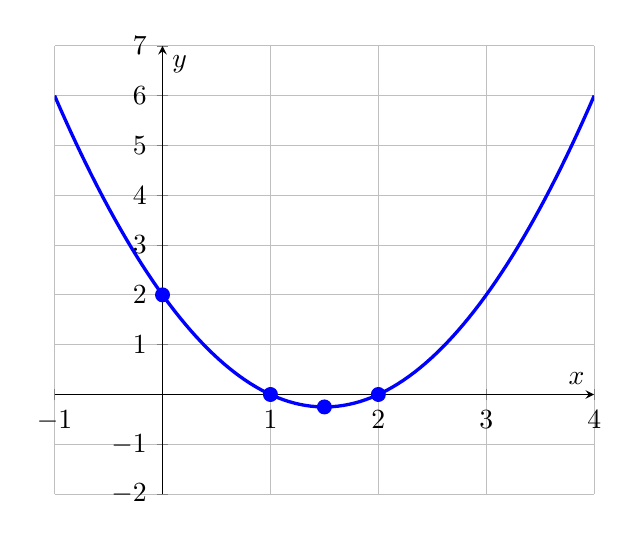
\begin{tikzpicture}
					\begin{axis}[
						axis lines = middle,
						xlabel = {$x$},
						ylabel = {$y$},
						xmin = -1, xmax = 4,
						ymin = -2, ymax = 7,
						xtick={-1,0,1,2,3,4},
						ytick={-2,-1,0,1,2,3,4,5,6,7},
						grid = both
						]
						
						% f(x) = x^2 - 3x + 2
						\addplot[
						domain=-1:4,
						samples=100,
						blue,
						very thick
						] {x^2 - 3*x + 2};
						
						% x-intercepts: (1,0) and (2,0)
						\addplot[
						only marks,
						mark=*,
						mark size=2.5pt,
						blue
						] coordinates {(1,0) (2,0)};
						
						% y-intercept: (0,2)
						\addplot[
						only marks,
						mark=*,
						mark size=2.5pt,
						blue
						] coordinates {(0,2)};
						
						% Vertex: (1.5,-1/4)
						\addplot[
						only marks,
						mark=*,
						mark size=2.5pt,
						blue
						] coordinates {(1.5,-0.25)};
						
					\end{axis}
				\end{tikzpicture}
				\item[(b)] 	Simplifying, we get $f(x)=(x^2+4x+4)-(x^2-4x+4)=8x$, so the function is not quadratic (it is linear).
				\item[(c)] 	Not quadratic (it is a rational function).
				\item[(d)] 
				Simplifying, we get $f(x)=3x-(x^2+3x+\dfrac{9}{4})=-x^2-\dfrac{9}{4}$, so the function is quadratic. The vertex form of the function is $f(x)=-(x-0)^2-\dfrac{9}{4}$.
				
				The domain of any quadratic function is $\mathbb{R}$, and the range is $\left( -\infty, -\dfrac{9}{4}\right]$.
				
				To find the $x$-intercept, we solve the equation $-x^2-\dfrac{9}{4}=0$, which is equivalent to $x^2=-\dfrac{9}{4}$. But this equation has no solutions and therefore there are no $x$-intercepts. To find the $y$-intercept, we set $x=0$ i.e. $-0^2-\dfrac{9}{4}=-\dfrac{9}{4}$, so the $y$-intercept is $(0,-\dfrac{9}{4})$.
				
				The function is increasing on $(-\infty,0)$ and it is decreasing on $(0,\infty)$.
				
				The function has a maximum at the point $\left(0,-\dfrac{9}{4}\right)$ and has no minimum.
				
				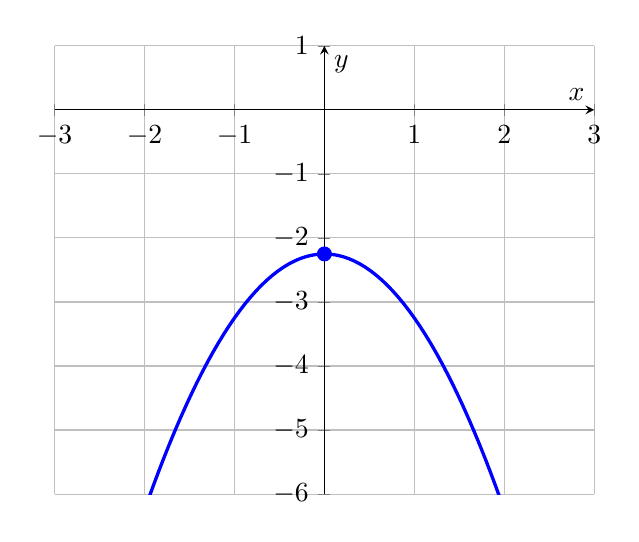
\begin{tikzpicture}
					\begin{axis}[
						axis lines = middle,
						xlabel = {$x$},
						ylabel = {$y$},
						xmin = -3, xmax = 3,
						ymin = -6, ymax = 1,
						xtick={-3,-2,-1,0,1,2,3},
						ytick={-6,-5,-4,-3,-2,-1,0,1},
						grid = both
						]
						
						% f(x) = 3x - (x + 3/2)^2
						\addplot[
						domain=-3:3,
						samples=100,
						blue,
						very thick
						] {3*x - (x + 1.5)^2};
						
						
						% Vertex: (0,-9/4)
						\addplot[
						only marks,
						mark=*,
						mark size=2.5pt,
						blue
						] coordinates {(0,-2.25)};
						
					\end{axis}
				\end{tikzpicture}
				\item[(e)] 
				Simplifying, we get $f(x)=(x^3+3x^2+3x+1)-(x^3+1)=3x^2+3x$, so the function is quadratic.
				
				To find the vertex form, we complete the square in the following way
				\begin{align*}
					3x^2+3x&=3(x^2+x)\\
					&=3(x^2+x+\left(\dfrac{1}{2}\right)^2-\left(\dfrac{1}{2}\right)^2)\\
					&=3(\left(x+\dfrac{1}{2}\right)^2-\dfrac{1}{4})\\
					&=3\left(x+\dfrac{1}{2}\right)^2-\dfrac{3}{4}.
				\end{align*}
				
				The domain of any quadratic function is $\mathbb{R}$, and the range is $\left[-\dfrac{3}{4},\infty \right).$
				
				To find the $x$-intercept, we solve the equation $3x^2+3x=0$, which is equivalent to $3x(x+1)=0$, i.e., $x=0, x=-1$. Thus, the function has two $x$-intercepts $(-1,0)$ and $(0,0)$. To find the $y$-intercept, we set $x=0$ i.e. $3\cdot0^2+3\cdot 0=0$, so the $y$-intercept is $(0,0)$.
				
				The function is decreasing on $(-\infty,-\dfrac{1}{2})$ and it is increasing on $(-\dfrac{1}{2},\infty)$.
				
				The function has a minimum at the point $\left(-\dfrac{1}{2},-\dfrac{3}{4}\right)$ and has no maximum.
				
				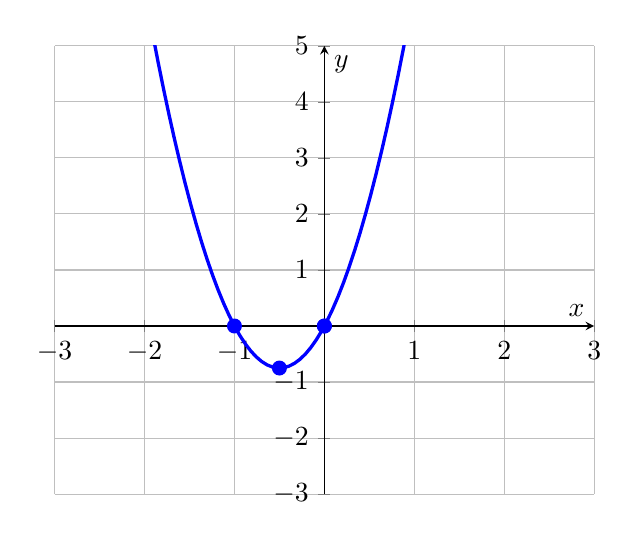
\begin{tikzpicture}
					\begin{axis}[
						axis lines = middle,
						xlabel = {$x$},
						ylabel = {$y$},
						xmin = -3, xmax = 3,
						ymin = -3, ymax = 5,
						xtick={-3,-2,-1,0,1,2,3},
						ytick={-3,-2,-1,0,1,2,3,4,5},
						grid = both
						]
						
						% f(x) = (x+1)^3 - (x+1)(x^2-x+1)
						% Simplified: f(x) = 3x^2 + 3x
						\addplot[
						domain=-3:3,
						samples=100,
						blue,
						very thick
						] {3*x^2 + 3*x};
						
						% x-intercepts: (-1,0) and (0,0)
						\addplot[
						only marks,
						mark=*,
						mark size=2.5pt,
						blue
						] coordinates {(-1,0) (0,0)};
						
						% y-intercept: (0,0)
						\addplot[
						only marks,
						mark=*,
						mark size=2.5pt,
						blue
						] coordinates {(0,0)};
						
						% Vertex: (-1/2,-3/4)
						\addplot[
						only marks,
						mark=*,
						mark size=2.5pt,
						blue
						] coordinates {(-0.5,-0.75)};
						
					\end{axis}
				\end{tikzpicture}
			\end{itemize}
		\end{solution}
		
		
		\item Find an equation for the line passing through the points $(1,2)$ and $(-1,0)$. Write your answer in the form $y=ax+b$.
		
		\begin{solution}
			The equation of a nonvertical line passing through two points $(x_1,y_1)$ and $(x_2,y_2)$ is $y-y_1=m(x-x_1)$, where the slope $m=\dfrac{y_2-y_1}{x_2-x_1}$. Note that it does not matter which point is first and which is second - they form the same line. For the given line, the slope is $m=\dfrac{2-0}{1-(-1)}=1$, so the equation of the line is $y-2=1(x-1)$, or $y=x+1$.
		\end{solution}
		\item Find an equation for the line passing through the points $(1,-5)$ and $(1,1)$. Write your answer in the form $ax+by+c=0$.
		\begin{solution}
			Notice that if you try to find the slope using the formula from above, you will get division by $0$. This indicates a vertical line (draw a sketch to confirm this). Since the $x$-coordinate of the two points does not change and is $1$, the equation of the line is $x=1$, or $x-1=0$.
		\end{solution}
		\item Find an equation for the line with slope $-1$, passing through the point $(-2,2)$. Write your answer in the form $y=ax+b$.
		\begin{solution}
			The equation of the line is $y-2=-1(x-(-2))$, which simplified is $y=-x$.
		\end{solution}
		\item Find an equation for the line with $y$-intercept 3 and slope $-2$. Write your answer in the form $ax+by+c=0$.
		\begin{solution}
			If the line has $y$-intercept $3$, it passes through the point $(0,3)$. Hence, the equation of the line is $y-3=-2(x-0)$, or $2x+y-3=0$.
		\end{solution}
		\item Find an equation for the line parallel to $2x-3y=1$, passing through the point $(1,-1)$. Write your answer in the form $ax+by+c=0$.
		\begin{solution}
			Parallel lines have the same slope. To find the slope of the given line, write it in the form $y=\dfrac{2}{3}x-\dfrac{1}{3}$. This line has slope $2/3$, and hence, any line parallel to it has slope $2/3$. Thus, the equation of the line is $y-(-1)=\dfrac{2}{3}(x-1)$, or $2x-3y-5=0$.
		\end{solution}
		\item Let $l_1$ be the line that passes through the points $(1,2)$ and $(-1,3)$. Find an equation for the line that is parallel to $l_1$ with $x$-intercept 2. Write your answer in the form $ax+by+c=0$.
		\begin{solution}
			The line is parallel to $l_1$, so it has the same slope $m=\dfrac{-1-1}{3-2}=-2$, and passes through the point $(2,0)$. Hence, its equation is $y-0=-2(x-2)$, or $2x+y-4=0$.
		\end{solution}
		\item Find the value of $k$ for which the line $2x-ky=1$
		\begin{enumerate}
			\item passes through the point $(1,-2)$.
			
			\item passes through the point $(1,0)$.
			
			\item passes through the point $(\dfrac{1}{2},0)$.
		
			\item is parallel to the line $2x+y=1$.
		
			\item is perpendicular to the line $2x+y=1$.
			
			\item is parallel to the line passing through the points $(1,-1)$ and $(3,-2)$.
		
			\item is perpendicular to the line $y=2$.
		
			\item is such that the nonzero coordinates of the $x$- and $y$-intercepts are equal.
			\end{enumerate}
			
			\begin{solution}
				\begin{itemize}
					\item[(a)] 	If a line passes through a point, then the coordinates of the point satisfy the equation of the line. Hence, we have $2\cdot1-k\cdot(-2)=1$. Solving for $k$, we get $k=-\dfrac{1}{2}$.
					\item[(b)] 	Similarly to part (a), we have $2\cdot 1-k\cdot 0=1$, or $2=1$. This equation does not have any solutions ($2=1$ is not a true statement for any $x$), so there is no $k$ that satisfies this condition.
					\item[(c)] In this case, we get the equation $2\cdot\dfrac{1}{2}-k\cdot0=1$, or $1=1$. Any real number $k \in \mathbb{R}$ satisfies this equation.
					\item[(d)] 	Transforming the equations to the form $y=mx+b$, we notice that the slope of the line $2x+y=1$ is $-2$ and the slope of the line $2x-ky=1$ is $\dfrac{2}{k}$ whenever $k\neq0$. Since the lines are parallel, the slopes are equal $-2=\dfrac{2}{k}$ and hence $k=-1$.
					\item[(e)] 	If two lines with slopes $m_1\neq 0$ and $m_2\neq 0$ are perpendicular, then $m_1\cdot m_2=-1$. The slope of $2x+y=1$ is $-2$ and hence $-2\cdot\dfrac{2}{k}=-1$. Solving this equation, we get $k=4$.
					\item[(f)] The slope of this line is $m=\dfrac{-2-(-1)}{3-1}=-\dfrac{1}{2}$. Hence, $-\dfrac{1}{2}=\dfrac{2}{k}$ and $k=-4$.
					\item[(g)] Since this line has slope $0$, we cannot use the equation from part (e). However, lines with slope $0$ are horizontal, so any line perpendicular to it has to be vertical. Thus, we need to find a $k$ for which $2x-ky=1$ is vertical. This happens when $k=0$.
					\item[(h)] 	The $x$-intercept is obtained by setting $y=0$. Hence, $2x=1$ and $x=\dfrac{1}{2}$. The $y$-intercept is obtained by setting $x=0$. Hence, $-ky=1$ and $y=-\dfrac{1}{k}$, provided $k\neq 0$ (note that when $k=0$, the line is vertical so it has no $y$-intercept). 
					
					Since the intercepts are equal, we set $\dfrac{1}{2}=-\dfrac{1}{k}$, so $k=-2$.
				\end{itemize}
			\end{solution}

			\item The bisector of a line segment is a line that passes through the midpoint of the line segment and is perpendicular to it. Find an equation of the bisector of the line segment that connects the points $(-3,-5)$ and $(1,1)$. Write the equation in the form $y=ax+b$.
			\begin{solution}
				The midpoint of the line segment has coordinates $\left(\dfrac{-3+1}{2},\dfrac{-5+1}{2}\right)=(-1,-2)$. Since the bisector is perpendicular to the line segment, $m_1\cdot m_2=-1$ holds for their respective slopes. The slope of the line segment is $m_1=\dfrac{1-(-5)}{1-(-3)}=\dfrac{3}{2}$. Therefore, we find the slope $m_2$ of the line by solving the equation $\dfrac{3}{2}\cdot m_2=-1$. Hence, $m_2=-\dfrac{2}{3}$, so the equation of the line is $y-(-2)=-\dfrac{2}{3}(x-(-1))$, or $y=-\dfrac{2}{3}x-\dfrac{8}{3}$.
			\end{solution}
	
		
		\item Determine whether the following statements are true or false. Justify your reasoning.
		\begin{enumerate}
			\item If a linear function has a negative $x$-intercept and a positive $y$-intercept, then its slope must be positive.
		
			\item If $f(x)=ax+b$ and $f(3)=f(7)$, then the graph of $f(x)$ is a horizontal line.
		
			\item If a quadratic function has a negative leading coefficient, then it has to have $x$-intercepts.
		
			\item The function $f(x)=-2(x-3)^2+8$ has a minimum at $(3,8)$.
		
			\item There exist two perpendicular lines with positive slopes.
		
			\item A vertical line has slope 0.
			
			\item The lines $ax+y=b$ and $ax-y=b$ are perpendicular for every $a\in\mathbb{R}\setminus\{0\}$.
			
			\item The lines $ax+y=b$ and $x-ay=b$ are perpendicular for every positive real number $a$.
			
		\end{enumerate}
		
		\begin{solution}
			\begin{itemize}
				\item[(a)] 	True. Say the $x$-intercept is $(a,0)$ and the $y$-intercept is $(0,b)$. Then the slope is $-b/a$, which is positive since $a$ is negative and $b$ is positive.
				\item[(b)] 	True. $f(3)=3a+b$ and $f(7)=7a+b$, which means $3a+b=7a+b \iff -4a=0 \iff a=0$. If the slope is 0, then the line is horizontal.
				\item[(c)] 	False. The graph of a quadratic function with a negative leading coefficient is open downwards, but the whole graph can be below the $x$-axis and therefore, have no $x$-intercepts. See for example the following function.
				
				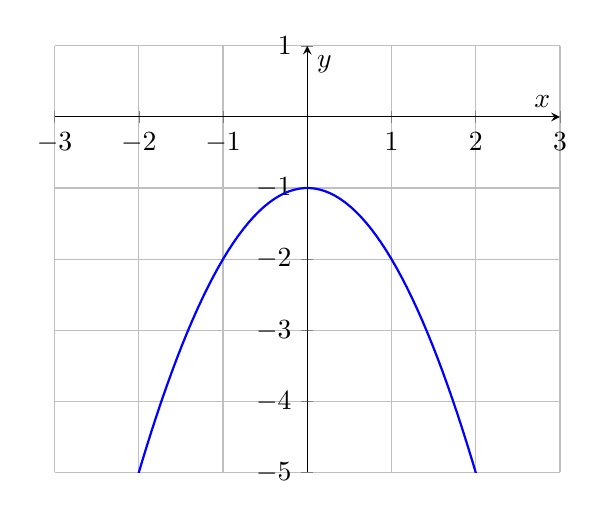
\begin{tikzpicture}
					\begin{axis}[
						axis lines=middle,
						xmin=-3, xmax=3,
						ymin=-5, ymax=1,
						xtick={-3,-2,-1,0,1,2,3},
						ytick={-5,-4,-3,-2,-1,0,1},
						grid=both,
						minor tick num=0,
						xlabel={$x$},
						ylabel={$y$},
						width=8cm,
						height=7cm,
						]
						\addplot[
						domain=-3:3,
						samples=100,
						thick,
						blue,
						] {-x^2-1};
					\end{axis}
				\end{tikzpicture}
				\item[(d)] 	False. The vertex form implies that the vertex is at $(3,8)$, however, the leading coefficient is $-2<0$, so the function has a maximum and not a minimum.
				\item[(e)] False. If the lines have slopes $m_1, m_2$, then $m_1\cdot m_2=-1$, which is not possible if both $m_1$ and $m_2$ are positive.
				\item[(f)] False. The slope of a line is only defined for non-vertical lines.
				\item[(g)] 	False. The first line has slope $-a$ and the second line has slope $a$. If the lines are perpendicular, then $-a\cdot a=-1$, which is true only for $a=\pm1$ and not for all nonzero real numbers.
				\item[(h)] True. The slope of the first line is $-a$ and the slope of the second line is $1/a$ (note that we have no issues with $a=0$ since $a$ is positive). Then $-a\cdot \dfrac{1}{a}=-1$, so the lines are perpendicular.
			\end{itemize}
		\end{solution}
		
	\end{enumerate}
	
	\newpage
	
	\section{Modeling with Linear and Quadratic Functions}
	

	\begin{enumerate}
		
		\item The temperature in a city is modeled by a linear function. At 6 a.m., the temperature is $42^\circ\text{F}$, and at 2 p.m., it is $66^\circ\text{F}$.
		
		\begin{enumerate}
			\item Find the average rate of change of the temperature with respect to time.
			\item Write a linear function $T(t)$ that models the temperature, where $t$ is the number of hours after 6 a.m.
			\item Use the model to predict the temperature at noon.
			\item Interpret the slope of the function in the context of the problem.
		\end{enumerate}
		
		\begin{solution}
			\begin{itemize} 
				\item[(a)] The average rate of change is $\dfrac{66-42}{14-6}=\dfrac{24}{8}=3$. Therefore, the temperature is increasing at an average rate of $3^\circ\text{F}$ per hour. 
				\item[(b)] Let $t$ represent the number of hours after 6 a.m. Since the temperature is $42^\circ\text{F}$ at $t=0$ and the slope is $3$, the linear model is $T(t)=3t+42.$ 
				\item[(c)] Noon is 6 hours after 6 a.m., so $T(6)=3(6)+42=60$. Therefore, the predicted temperature at noon is $60^\circ\text{F}$. 
				\item[(d)] The slope is $3$, which means that the temperature is increasing by approximately $3^\circ\text{F}$ for each hour after 6 a.m. 
				\end{itemize}
		\end{solution}
		
		\item A town's population was 18400 in 2015 and 21700 in 2025. Assume the population changes at a constant rate.
		
		\begin{enumerate}
			\item Find the average rate of change of the population.
			\item Write a linear model $P(t)$, where $t$ is the number of years after 2015.
			\item Use the model to predict the population in 2030.
			\item According to the model, when will the population reach 25,000?
		\end{enumerate}
		
		\begin{solution}
			\begin{itemize} 
				\item[(a)] The average rate of change is $\dfrac{21700-18400}{2025-2015} = \dfrac{3300}{10} =330$. Therefore, the population is increasing at a rate of $330$ people per year. 
				\item[(b)] Let $t$ represent the number of years after 2015. Since $P(0)=18400$ and the slope is $330$, the linear model is $P(t)=330t+18400$.
				\item[(c)] The year 2030 corresponds to $t=15$. Thus, $P(15)=330(15)+18400 = 4950+18400 =23350$. Therefore, the predicted population in 2030 is $23350$. 
				\item[(d)] To determine when the population will reach 25000, solve $25000=330t+18400$. Thus, $6600=330t$ and $t=20$. Therefore, according to the model, the population will reach 25000 in $2015+20=2035$. 
				\end{itemize}
		\end{solution}
		
		\item A concert venue can sell 2,000 tickets. When tickets are priced at \$40, an average of 1,800 tickets are sold. For every \$5 increase in ticket price, 100 fewer tickets are sold.
		
		Let $x$ represent the number of \$5 price increases.
		
		\begin{enumerate}
			\item Write a function for the ticket price.
			\item Write a function for the number of tickets sold.
			\item Find a quadratic function $R(x)$ representing the revenue.
			\item What ticket price produces the greatest revenue?
			\item What is the maximum revenue?
		\end{enumerate}
		
		\begin{solution}
			\begin{itemize} 
				\item[(a)] The ticket price increases by \$5 for each increase, so the price function is $p(x)=40+5x$. 
				\item[(b)] The number of tickets sold decreases by 100 for each increase, so the number of tickets sold is $q(x)=1800-100x$.
				\item[(c)] The revenue is given by $R(x)=p(x)q(x)$. Therefore, $R(x)=(40+5x)(1800-100x)$. Expanding, $R(x)=-500x^2+5000x+72000$. 
				\item[(d)] Since the revenue function is a quadratic function that opens downward, its maximum occurs at the vertex. The $x$-coordinate of the vertex is $x=-\dfrac{b}{2a} =-\dfrac{5000}{2(-500)} =5$. Thus, the ticket price that produces the greatest revenue is $p(5)=40+5(5)=65$. Therefore, the ticket price should be \$65. 
				\item[(e)] The maximum revenue is $R(5)=-500(5)^2+5000(5)+72000=-12500+25000+72000 =84500$. Therefore, the maximum revenue is \$84500. 
			\end{itemize}
		\end{solution}
		
		\item A company produces and sells a product. The fixed cost is \$8,000, and the variable cost is \$12 per unit. Each unit is sold for \$32.
		
		\begin{enumerate}
			\item Write the cost function $C(x)$.
			\item Write the revenue function $R(x)$.
			\item Find the profit function $P(x)$.
			\item How many units must be sold to break even?
			\item What is the company's profit when 1000 units are sold?
		\end{enumerate}
		\begin{solution}
			\begin{itemize}
				\item[(a)] The cost consists of a fixed cost of \$8000 and a variable cost of \$12 per unit. Therefore, $C(x)=8000+12x$, where $x$ is the number of products.
				\item[(b)] The revenue is the price per unit multiplied by the number of units sold: $ R(x)=32x$. 
				\item[(c)] The profit is the revenue minus the cost: $P(x)=R(x)-C(x)$. Therefore, $P(x)=32x-(8000+12x)$ and $P(x)=20x-8000$.
				\item[(d)] To find the break-even point, set the profit equal to zero: $20x-8000=0$. Thus, $20x=8000$ and $x=400$. Therefore, the company must sell $400$ units to break even. 
				\item[(e)] When $1000$ units are sold, $P(1000)=20(1000)-8000 =20000-8000 = 12000$. Therefore, the company's profit is \$12000.
			\end{itemize}
		\end{solution}
		
		\item The height of an object dropped from a building is modeled by $h(t)=-16t^2+144$, where $h(t)$ is measured in feet and $t$ is measured in seconds.
		
		\begin{enumerate}
			\item What is the initial height of the object?
			\item What is the height of the object after 2 seconds?
			\item When does the object hit the ground?
			\item What is the average rate of change of the height between $t=1$ and $t=2$?
			\item Interpret the meaning of the average rate of change.
		\end{enumerate}
		
		\begin{solution}
			\begin{itemize}
				\item[(a)] The initial height occurs when $t=0$: $ h(0)=-16(0)^2+144=144$. Therefore, the object was initially $144$ feet above the ground. 
				\item[(b)] After 2 seconds, $h(2)=-16(2)^2+144 =-64+144 = 80$. Therefore, the height after 2 seconds is $80$ feet. 
				\item[(c)] The object hits the ground when $h(t)=0$. Thus, $-16t^2+144=0$. Dividing by $-16$ gives $t^2=9.$ Therefore, $t=\pm3$. Since time cannot be negative, $t=3$. Therefore, the object hits the ground after $3$ seconds. 
				\item[(d)] The average rate of change between $t=1$ and $t=2$ is $\dfrac{h(2)-h(1)}{2-1}$. We have $h(2)=80$ and $h(1)=-16(1)^2+144=128$. Therefore, $\dfrac{80-128}{2-1}=-48$. Thus, the average rate of change is $-48$ feet per second. 
				\item[(e)] The negative sign indicates that the height is decreasing. Therefore, between $t=1$ and $t=2$, the object's height decreases at an average rate of $48$ feet per second.
			\end{itemize}
		\end{solution}
		
		\item A ball is thrown vertically upward from a platform 6 feet above the ground with an initial velocity of 64 ft/s. Its height is modeled by $h(t)=-16t^2+64t+6$.
		
		\begin{enumerate}
			\item What is the initial height of the ball?
			\item What is the height after 2 seconds?
			\item When does the ball reach its maximum height?
			\item What is the maximum height?
			\item When does the ball hit the ground?
		\end{enumerate}
		
		\begin{solution}
			\begin{itemize}
				\item[(a)] The initial height occurs when $t=0$: $ h(0)=-16(0)^2+64(0)+6=6$. Therefore, the initial height of the ball is $6$ feet. 
				\item[(b)] After 2 seconds, $h(2)=-16(2)^2+64(2)+6$. Thus, $h(2)=-64+128+6=70$. Therefore, the height after 2 seconds is $70$ feet. 
				\item[(c)] Since the height function is a quadratic function that opens downward, the maximum occurs at the vertex. The time at which the ball reaches its maximum height is $t=-\dfrac{b}{2a} =-\dfrac{64}{2(-16)} =2$. Therefore, the ball reaches its maximum height after $2$ seconds. 
				\item[(d)] The maximum height is $h(2)=70.$ Therefore, the maximum height is $70$ feet. 
				\item[(e)] The ball hits the ground when $h(t)=0$. Thus, $-16t^2+64t+6=0$. Dividing by $-2$ gives $8t^2-32t-3=0$. Using the quadratic formula, $$ t=\dfrac{-(-32)\pm\sqrt{(-32)^2-4(8)(-3)}}{2(8)}. $$ Therefore, $t=\dfrac{32\pm\sqrt{1120}}{16} =\dfrac{32\pm4\sqrt{70}}{16} =\dfrac{8\pm\sqrt{70}}{4}$. Since time must be positive, $t=\dfrac{8+\sqrt{70}}{4}\approx4.09.$ Therefore, the ball hits the ground approximately $4.09$ seconds after it is thrown.
			\end{itemize}
		\end{solution}
		
	\end{enumerate}
	
	
	
	
	\newpage
	
	\section{Algebraic Functions}
	\begin{enumerate}
		
		\item Find the implied domain of the following power functions.
		\begin{enumerate}
			\item $f_1(x)=\sqrt{2}x^{2/3}$
			
			\item $f_2(x)=-3x^{-3}$
		
			\item $f_3(x)=2x^{-5/2}$
		
			\item $f_4(x)=\dfrac{x^{1/4}}{4}$
			
		\end{enumerate}
		Then find $f_1(-8), f_2(-3), f_3(4), f_4(16)$.
		\begin{solution}
			\begin{itemize}
				\item[(a)] The domain is $\mathbb{R}$.
				\item[(b)] The domain is $\mathbb{R}\setminus \{0\}$.
				\item[(c)] The domain is $(0,\infty)$.
				\item[(d)] The domain is $[0,\infty)$.
			\end{itemize}
			$$f_1(-8)=\sqrt{2}(-8)^{2/3}=\sqrt{2}((-2)^3)^{2/3}=\sqrt{2} (-2)^2=4\sqrt{2}$$
			
			$$f_2(-3)=-3\cdot(-3)^{-3}=-3\cdot \dfrac{1}{(-3)^3}=-3\cdot \dfrac{1}{-27}=\dfrac{1}{9}$$
			
			$$f_3(4)=2\cdot 4^{-5/2}=2\cdot (2^2)^{-5/2}=2\cdot 2^{(-5)}=2^{-4}=\dfrac{1}{16}$$
			
			$$f_4(16)=\dfrac{16^{1/4}}{4}=\dfrac{(2^4)^{1/4}}{4}=\dfrac{2}{4}=\dfrac{1}{2}.$$
		\end{solution}
		
		\item Simplify the expression to one involving only positive exponents. Assume that everything is well-defined.
		\begin{enumerate}
			\item $\left(\dfrac{x^{-1/4}y}{xz^2}\right)^{-4}$
			
			\item $\dfrac{(x^3y)^{-1}(8^{-1}x^4y^3)}{(2x^2y^{-3})^{-2}}$
		
		\end{enumerate}
		\begin{solution}
			\begin{itemize}
				\item[(a)] 	$\left(\dfrac{x^{-1/4}y}{xz^2}\right)^{-4}=\dfrac{(x^{-1/4})^{-4}y^{-4}}{x^{-4}(z^2)^{-4}}=\dfrac{xy^{-4}}{x^{-4}z^{-8}}=\dfrac{xx^4z^8}{y^4}=\dfrac{x^5z^8}{y^4}.$
				\item[(b)] $\dfrac{(x^3y)^{-1}(8^{-1}x^4y^3)}{(2x^2y^{-3})^{-2}}=\dfrac{x^{-3}y^{-1}8^{-1}x^4y^3}{2^{-2}x^{-4}y^6}=\dfrac{xy^28^{-1}}{2^{-2}x^{-4}y^6}=\dfrac{xx^42^2}{8y^{6-2}}=\dfrac{x^5}{2y^4}.$
			\end{itemize}
		\end{solution}
		\item Let $n$ and $x$ be positive integers. Write the following expression $\dfrac{\sqrt[3]{x^{6n}x^{-3n-9}}}{\sqrt{x^{2(n+2)}}}$ in the form $x^k$, for some integer $k$. 
		\begin{solution}
			$\dfrac{\sqrt[3]{x^{6n}x^{-3n-9}}}{\sqrt{x^{2(n+2)}}}=\dfrac{x^{6n/3}x^{(-3n-9)/3}}{x^{2(n+2)/2}}=\dfrac{x^{2n}x^{-n-3}}{x^{n+2}}=\dfrac{x^{2n-n-3}}{x^{n+2}}=\dfrac{x^{n-3}}{x^{n+2}}=x^{(n-3)-(n+2)}=x^{-5}.$
		\end{solution}
		
		\item Determine the degree, leading coefficient, leading term and constant term of the following polynomials.
		\begin{enumerate}
			\item $-(1-x)^2+2(x-1)(2x+1)-(x-2)(x+2)$

			\item $(x-2)(x^2+2x+4)-(x-2)^3$
		
			\item $(x^2+x-6)^2-2x(x+3)(x^2+1)$
			
		\end{enumerate}
		
		\begin{solution}
			\begin{itemize}
				\item[(a)] 	\begin{align*}
					&-(1-x)^2+2(x-1)(2x+1)-(x-2)(x+2)\\&=-(1-2x+x^2)+2(2x^2+x-2x-1)-(x^2-4)\\
					&=-1+2x-x^2+4x^2+2x-4x-2-x^2+4\\
					&=2x^2+1
				\end{align*}
				The degree of the polynomial is 2, the leading coefficient is $2$, the leading term is $2x^2$ and the constant term is $1$.
				\item[(b)] 	\begin{align*}
					&(x-2)(x^2+2x+4)-(x-2)^3\\
					&=(x^3-2^3)-(x^3-6x^2+12x-8)\\
					&=x^3-8-x^3+6x^2-12x+8\\
					&=6x^2-12x
				\end{align*}
				The degree of the polynomial is 2, the leading coefficient is 6, the leading term is $6x^2$ and the constant term is $0$.
				\item[(c)] 	\begin{align*}
					&(x^2+x-6)^2-2x(x+3)(x^2+1)\\
					&=(x^4+x^2+6^2+2x^3-12x^2-12x)-2x(x^3+x+3x^2+3)\\
					&=x^4+2x^3-11x^2-12x+36-2x^4-2x^2-6x^3-6x\\
					&=-x^4-4x^3-13x^2-18x+36
				\end{align*}
				The degree of the polynomial is 4, the leading coefficient is -1, the leading term is $-x^4$ and the constant term is 36.
			\end{itemize}
		\end{solution}
		
		\item Determine the values of $a,b,c$ so that the polynomials $f(x)$ and $g(x)$ are equal.\begin{enumerate}
			\item 
			$
			f(x)=2(x-3)^2-4(x+1)
			$
			
			$
			g(x)=(a-1)x^2+(b+5)x+c.
			$
			
		
			
			\item $f(x)=(x-3)(2x^2-4x+5)+(x+2)(x^2-3x+1)$
			
			$g(x)=(a+b)x^3+(2a-c)x^2+(b+3c)x+11.
			$
			
		
		\end{enumerate}
		
		\begin{solution}
			\begin{itemize}
				\item[(a)] 	Two polynomials are equal if the corresponding coefficients are equal. We have
				$f(x)=2x^2-12x+18-4x-4=2x^2-16x+14$, so we get 
				$a-1=2, b+5=-16, c=14$, i.e. $a=3,b=-21,c=14$.
				\item[(b)] We have $f(x)=2x^3-4x^2+5x-6x^2+12x-15+x^3-3x^2+x+2x^2-6x+2=3x^3-11x^2+12x-13$. Thus $a+b=3,2a-c=-11,b+3c=12$, i.e., $a=-\dfrac{24}{5},b=\dfrac{39}{5},c=\dfrac{7}{5}$.
			\end{itemize}
		\end{solution}
		
		\item Find the (real) roots of the following polynomials.
		\begin{enumerate}
			\item $x^3-2x^2-x+2$
			
			\item $x^3-4x^2+x+6$
			
			\item $x^4+x^3+2x-4$
		
		\end{enumerate}
		
		\begin{solution}
			\begin{itemize}
				\item[(a)] 	$x^3-2x^2-x+2=0 \iff x^2(x-2)-(x-2)=0\iff (x-2)(x^2-1)=0\iff (x-2)(x-1)(x+1)=0$ and therefore, the roots are $2,1,-1$.
				\item[(b)] 	This polynomial does not factor as easily as the previous one. Using the Integer Root theorem, the possible integer solutions to the equation $x^3-4x^2+x+6=0$ are the divisors of $6$, i.e., $\pm1,\pm2,\pm3,\pm6$. Notice that $-1$ is one solution. Then use long division of polynomials to divide the given polynomial by $x-(-1)=x+1$:
				
				$$
				\begin{array}{r@{}l}
					& \underline{x^2-5x+6} \\
					x+1\,\big)\,& x^3-4x^2+x+6 \\[1mm]
					& \underline{x^3+x^2} \\[-1mm]
					& \phantom{x^3+}(-5x^2+x) \\[1mm]
					& \underline{\phantom{x^3+}(-5x^2-5x)} \\[-1mm]
					& \phantom{x^3-4x^2+}(6x+6) \\[1mm]
					& \underline{\phantom{x^3-4x^2+}(6x+6)} \\[-1mm]
					& 0
				\end{array}.
				$$
				Next, we solve the equation $x^2-5x+6=0\iff(x-3)(x-2)=0\iff x=3,x=2$.
				
				Thus, the roots of the polynomial are $-1,2,3$.
				\item[(c)] 	Similarly, we notice that 1 is a solution to the equation $x^4+x^3+2x-4=0$. We use long division to divide the given polynomial by $x-1$:
				
				$$
				\begin{array}{r@{}l}
					& \underline{x^3+2x^2+2x+4} \\
					x-1\,\big)\,& x^4+x^3+0x^2+2x-4 \\[1mm]
					& \underline{x^4-x^3} \\[-1mm]
					& \phantom{x^4+}(2x^3+0x^2) \\[1mm]
					& \underline{\phantom{x^4+}(2x^3-2x^2)} \\[-1mm]
					& \phantom{x^4+x^3+}(2x^2+2x) \\[1mm]
					& \underline{\phantom{x^4+x^3+}(2x^2-2x)} \\[-1mm]
					& \phantom{x^4+x^3+0x^2+}(4x-4) \\[1mm]
					& \underline{\phantom{x^4+x^3+0x^2+}(4x-4)} \\[-1mm]
					& 0
				\end{array}.
				$$
				
				Next, we solve the equation $x^3+2x^2+2x+4=0 \iff x^2(x+2)+2(x+2)=0\iff (x^2+2)(x+2)=0$. Since $x^2+2=0$ has no real solutions, the only roots of the polynomial are 1 and -2.
				
				Note that if $x^3+2x^2+2x+4=0$ was not easily factorizable, we would use the integer root theorem and long division, as previously. 
			\end{itemize}
		\end{solution}
		
		\item Classify the following functions as one of the following: power functions, polynomial functions, rational functions, algebraic functions that are none of the previous types. Note that some functions belong to more than one function class.
		\begin{enumerate}
			\item $f(x)=\sqrt{x}$
		
			\item $f(x)=\sqrt{\pi}$
		
			\item $f(x)=x^2$
		
			\item $f(x)=2(x^{3/2}+1)$
		
			\item $f(x)=2x^{5/2}-x^{3/2}+1$
		
			\item $f(x)=\dfrac{1+x}{1+x^2}$
		
			\item $f(x)=\dfrac{1+x}{1+\sqrt{x}}$
		
		\end{enumerate}
		
		\begin{solution}
			\begin{itemize}
				\item[(a)] Power function.
				\item[(b)] 	Polynomial function, power function, rational function.
				\item[(c)] Polynomial function, power function, rational function.
				\item[(d)] Algebraic function.
				\item[(e)] 	Algebraic function.
				\item[(f)] Rational function.
				\item[(g)] 	Algebraic function.
			\end{itemize}
		\end{solution}
		
		\item Find the (implied) domain and the zeroes (if any) of the following functions.
		\begin{enumerate}
			\item $f(x)=x^2-x+2$
		
			\item $f(x)=\dfrac{x^2-x-2}{5}$
		
			\item $f(x)=\dfrac{x-2}{2x^2-3x+1}$
		
			\item $f(x)=\dfrac{x-2}{x^2-4}$
		
			\item $f(x)=\dfrac{x^2-1}{x^3-x^2+x-1}$
			
			\item $f(x)=\dfrac{x^2+1}{x^3-2x+1}$
			
	
		\end{enumerate}
		
		\begin{solution}
			\begin{itemize}
				\item[(a)] 	This is a polynomial function (quadratic, to be specific) and therefore, the domain is $\mathbb{R}$.
				
				To find the zeroes, we have to solve the equation $x^2-x+2=0$. However, this equation has no real solutions, so the function has no zeroes.
				\item[(b)] This is also a polynomial function and hence the domain is $\mathbb{R}$. 
				
				The zeroes are $-1$ and $2$, obtained by solving the equation $\dfrac{x^2-x-2}{5}=0$.
				\item[(c)] This is a rational function that is defined for all real numbers such that $2x^2-3x+1\neq0$. The solutions to this equation are $x=1/2$ and $x=1$ and hence, the domain of the function is $\mathbb{R} \setminus \{1,\dfrac{1}{2}\}$.
				
				$\dfrac{x-2}{2x^2-3x+1}=0$ whenever $x-2=0$ or $x=2$. Therefore, the function has one zero $2$. 
				\item[(d)] $x^2-4=0$ whenever $x=\pm 2$. Therefore, the domain of the function is $\mathbb{R}\setminus \{-2,2\}$.
				
				$\dfrac{x-2}{x^2-4}=0$ whenever $x-2=0$ or $x=2$. However, $2$ is not in the domain of the function, and therefore the function has no zeroes.
				\item[(e)]	$$x^3-x^2+x-1=0$$
				$$x^2(x-1)+(x-1)=0$$
				$$(x-1)(x^2+1)=0$$
				$$x=1$$
				since $x^2+1\neq 0$ for any real number $x$. Therefore, the domain of the function is $\mathbb{R}\setminus \{1\}$.
				
				$x^2-1=0$ whenever $x^2=1$ i.e., whenever $x=\pm1$. However, $1$ is not in the domain of the function, and hence, the only zero of the function is $-1$.
				\item[(f)] 	To find the domain, we need to solve the equation $x^3-2x+1=0$. First, notice that $x=1$ is a solution. Then, using long division, we conclude that $x^3-2x+1=(x-1)(x^2+x-1)$. Solving $x^2+x-1=0$, we get $x=\dfrac{-1\pm\sqrt{5}}{2}$. Thus the domain of the function is $\mathbb{R}\setminus \{1,\dfrac{-1\pm\sqrt{5}}{2}\}$.
				
				To find the zeroes, we need to solve $\dfrac{x^2+1}{x^3-2x+1}=0$, which is equivalent to $x^2+1=0$. This equation has no real solutions and hence, the function has no zeroes.
			\end{itemize}
		\end{solution}
		
		\item Determine whether the following statements are true or false. Justify your reasoning.
		\begin{enumerate}
				\item The functions
				$
				f(x)=\dfrac{x^2-4}{x-2}$ and $g(x)=x+2
				$
				are equal functions.
				
				\item The domain of $f(x)=\dfrac{\sqrt{x-2}}{x-5}$
				is $[2,5)\cup(5,\infty)$.
			
				\item The function $f(x)=x^{5/2}-x^{3/2}$ is a power function.
			
				\item The function $f(x)=\dfrac{x^3+x^2}{x}$ is a polynomial function.
				
				\item The function $f(x)=x^{5/3}$ is defined for every real number $x$.				
				
				\item The function $f(x)=x^{-2/3}$ is defined at $x=0$.
				
				
				\item Every polynomial function is an algebraic function.
				
				\item Every algebraic function is a polynomial function. 
				
				
				\item The polynomial $f(x)=x^4-16$
				has exactly two real zeroes.
			
				\item If $f(x)=x^{2/3}$, then $f(-8)=4.$
			
				\item If $f(x)=x^{3/2}$, then $f(-4)=-8.$
				
		\end{enumerate}
		
	\end{enumerate}
	
	\begin{solution}
		\begin{itemize}
			\item[(a)] 	False. The domain of $f(x)$ is $\mathbb{R}\setminus\{2\}$ and the domain of $g(x)$ is $\mathbb{R}$.
			\item[(b)] True. The numerator is a square root function, which is defined for all $x$ such that $x-2\geq0\iff x\geq 2$. However, the denominator cannot be 0, so we have $x-5\neq0 \iff x\neq 5$. Thus, the domain is $[2,5)\cup(5,\infty)$.
			\item[(c)] False. $f(x)$ cannot be written in the form $Ax^k$, for $A\in\mathbb{R}$ and $k$ a rational number.
			\item[(d)] False. This is a rational function, but it is not polynomial (even though the expression simplifies to $x^2+x$ for $x\neq0$).
			\item[(e)] True. Any power function of the form $f(x)=Ax^k$, where $k$ is a positive rational number with an odd denominator, has domain $\mathbb{R}$.
			\item[(f)] False. The power functions of the form $f(x)=Ax^k$, where $k$ is a negative rational number, have domain $\mathbb{R}\setminus\{0\}$.
			\item[(g)] True. The polynomial functions are a subclass of the algebraic functions.
			\item[(h)]	False. For example, the function $f(x)=\sqrt{x}$ is algebraic but not polynomial.
			\item[(i)] True. $x^4-16=0\iff (x^2-4)(x^2+4)=0\iff (x-2)(x+2)(x^2+4)=0\iff x=2,x=-2$ (since $x^2+4=0$ has no real solutions). Thus, the only real zeroes of the polynomial are $-2$ and 2.
			\item[(j)] True. $f(-8)=(-8)^{2/3}=((-2)^3)^{2/3}=(-2)^2=4$.
			\item[(k)] False. The function is not defined for negative numbers.
			
		\end{itemize}
	\end{solution}
	
	
	\newpage
		\section{Transformations and Symmetry}
	
	\begin{enumerate}
		\item The graph of the function $f(x)$ is given below.
		
		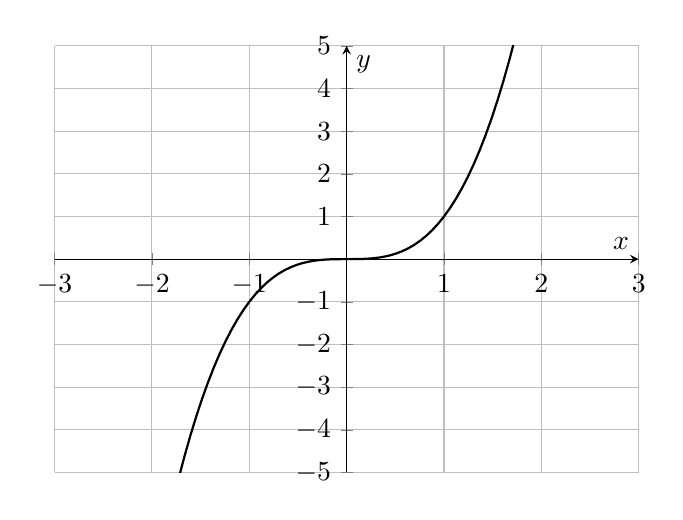
\begin{tikzpicture}
			\begin{axis}[
				axis lines=middle,
				xmin=-3, xmax=3,
				ymin=-5, ymax=5,
				xlabel={$x$},
				ylabel={$y$},
				xtick={-3,-2,-1,0,1,2,3},
				ytick={-5,-4,-3,-2,-1,0,1,2,3,4,5},
				grid=both,
				width=9cm,
				height=7cm,
				]
				
				\addplot[
				domain=-3:3,
				samples=100,
				thick,
				black
				] {x^3};
				
			\end{axis}
		\end{tikzpicture}
		
		 Sketch the graphs of the following functions and state the transformation of $f(x)$.
		\begin{enumerate}
			\item $f(x)+1, f(x)-1, f(x+1), f(x-1)$
			\item $2f(x), \dfrac{1}{2}f(x), f(2x), f(\dfrac{1}{2}x)$
			\item $-f(x),f(-x)$
		\end{enumerate}
		\begin{solution}
			\begin{itemize}
				\item[(a)] 
				
				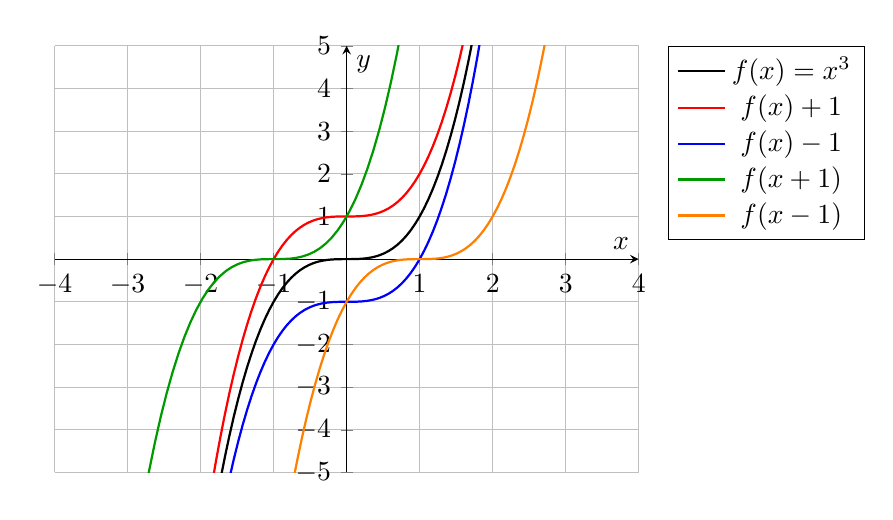
\begin{tikzpicture}
					\begin{axis}[
						axis lines=middle,
						xmin=-4, xmax=4,
						ymin=-5, ymax=5,
						xlabel={$x$},
						ylabel={$y$},
						xtick={-4,-3,-2,-1,0,1,2,3,4},
						ytick={-5,-4,-3,-2,-1,0,1,2,3,4,5},
						grid=both,
						width=9cm,
						height=7cm,
						legend style={
							at={(1.05,1)},
							anchor=north west
						}
						]
						
						% f(x) = x^3
						\addplot[
						domain=-3:3,
						samples=100,
						thick,
						black
						] {x^3};
						\addlegendentry{$f(x)=x^3$}
						
						% f(x) + 1
						\addplot[
						domain=-3:3,
						samples=100,
						thick,
						red
						] {x^3+1};
						\addlegendentry{$f(x)+1$}
						
						% f(x) - 1
						\addplot[
						domain=-3:3,
						samples=100,
						thick,
						blue
						] {x^3-1};
						\addlegendentry{$f(x)-1$}
						
						% f(x + 1)
						\addplot[
						domain=-4: 4,
						samples=100,
						thick,
						green!60!black
						] {(x+1)^3};
						\addlegendentry{$f(x+1)$}
						
						% f(x - 1)
						\addplot[
						domain=-2:4,
						samples=100,
						thick,
						orange
						] {(x-1)^3};
						\addlegendentry{$f(x-1)$}
						
					\end{axis}
				\end{tikzpicture}
				
				\item[(b)] 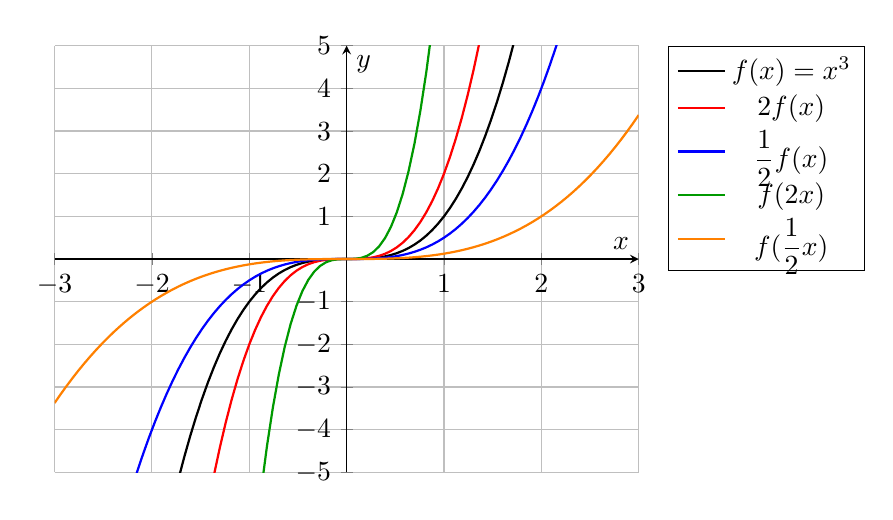
\begin{tikzpicture}
					\begin{axis}[
						axis lines=middle,
						xmin=-3, xmax=3,
						ymin=-5, ymax=5,
						xlabel={$x$},
						ylabel={$y$},
						xtick={-3,-2,-1,0,1,2,3},
						ytick={-5,-4,-3,-2,-1,0,1,2,3,4,5},
						grid=both,
						width=9cm,
						height=7cm,
						legend style={
							at={(1.05,1)},
							anchor=north west
						}
						]
						
						% f(x) = x^3
						\addplot[
						domain=-3:3,
						samples=100,
						thick,
						black
						] {x^3};
						\addlegendentry{$f(x)=x^3$}
						
						% 2f(x)
						\addplot[
						domain=-3:3,
						samples=100,
						thick,
						red
						] {2*x^3};
						\addlegendentry{$2f(x)$}
						
						% (1/2)f(x)
						\addplot[
						domain=-3:3,
						samples=100,
						thick,
						blue
						] {0.5*x^3};
						\addlegendentry{$\dfrac{1}{2}f(x)$}
						
						% f(2x)
						\addplot[
						domain=-3:3,
						samples=100,
						thick,
						green!60!black
						] {(2*x)^3};
						\addlegendentry{$f(2x)$}
						
						% f(1/2 x)
						\addplot[
						domain=-3:3,
						samples=100,
						thick,
						orange
						] {(0.5*x)^3};
						\addlegendentry{$f(\dfrac{1}{2}x)$}
						
					\end{axis}
				\end{tikzpicture}
				
				\item[(c)]
				
				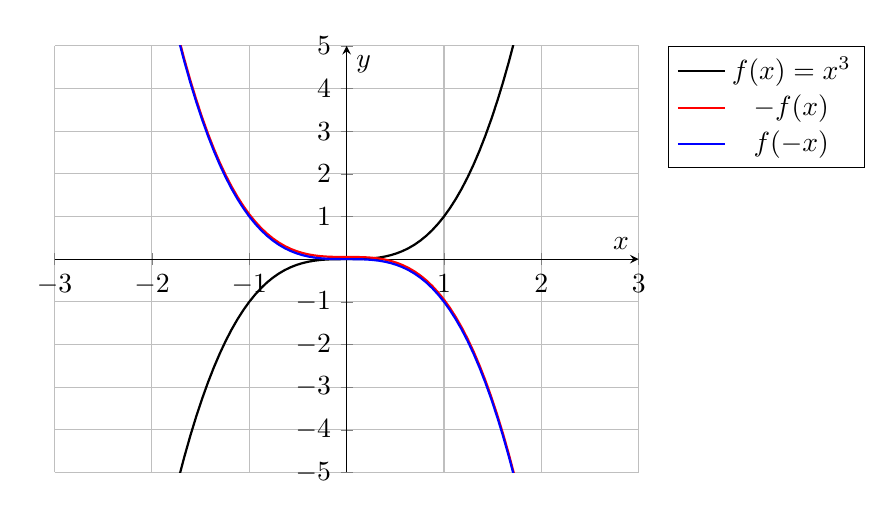
\begin{tikzpicture}
					\begin{axis}[
						axis lines=middle,
						xmin=-3, xmax=3,
						ymin=-5, ymax=5,
						xlabel={$x$},
						ylabel={$y$},
						xtick={-3,-2,-1,0,1,2,3},
						ytick={-5,-4,-3,-2,-1,0,1,2,3,4,5},
						grid=both,
						width=9cm,
						height=7cm,
						legend style={
							at={(1.05,1)},
							anchor=north west
						}
						]
						
						% f(x) = x^3
						\addplot[
						domain=-3:3,
						samples=100,
						thick,
						black
						] {x^3};
						\addlegendentry{$f(x)=x^3$}
						
						% -f(x) = -x^3, fully red
						\addplot[
						domain=-3:3,
						samples=100,
						thick,
						red
						] {-x^3+0.05};
						\addlegendentry{$-f(x)$}
						
						% f(-x) = -x^3, fully blue
						\addplot[
						domain=-3:3,
						samples=100,
						thick,
						blue
						] {(-x)^3};
						\addlegendentry{$f(-x)$}
						
					\end{axis}
				\end{tikzpicture}
			\end{itemize}
		\end{solution}
		\item The graph of the function $f(x)$ is given below.
		
		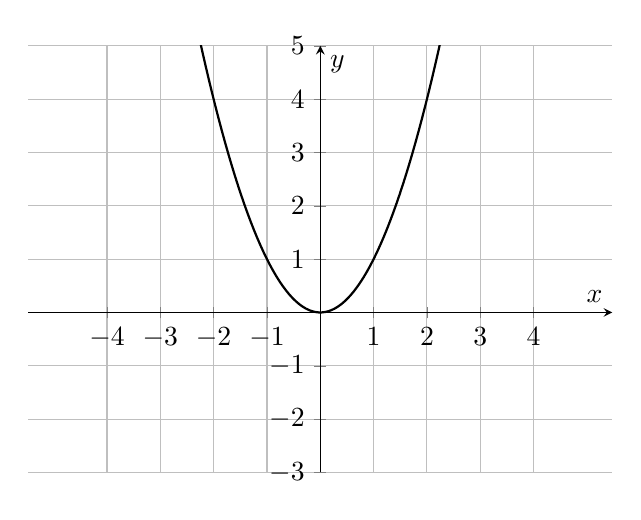
\begin{tikzpicture}
			\begin{axis}[
				axis lines=middle,
				xmin=-3, xmax=3,
				ymin=-3, ymax=5,
				xlabel={$x$},
				ylabel={$y$},
				xtick={-4,-3,-2,-1,0,1,2,3,4},
				ytick={-3,-2,-1,0,1,2,3,4,5},
				grid=both,
				width=9cm,
				height=7cm,
				axis equal
				]
				
				\addplot[
				domain=-3:3,
				samples=100,
				thick,
				black
				] {x^2};
				
				
			\end{axis}
		\end{tikzpicture}
		
		 Sketch the graphs of the following functions and explain which transformations of the graph of $f(x)$, and in what order, produce the graph of $g(x)$.
		\begin{enumerate}
			\item $g(x)=-2f(x-1)+1$
			\item $g(x)=\dfrac{1}{2}f(2x+3)-2$
		\end{enumerate}
		\begin{solution}
			\begin{itemize}
				\item[(a)] Shift to the right by 1 $\Rightarrow$ Reflection about the $x$-axis $\Rightarrow$ Stretch vertically by a factor of 2 $\Rightarrow$ shift up by 1.
				
				
				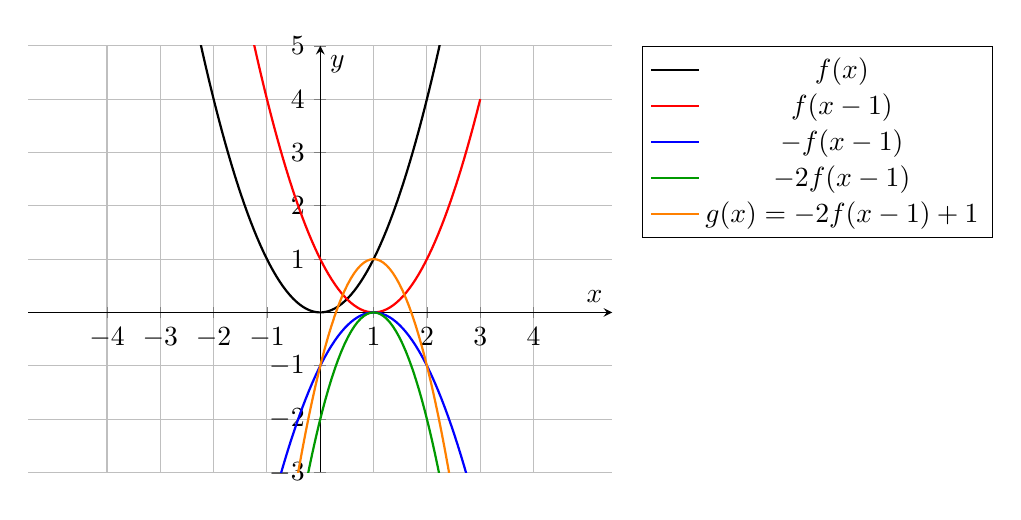
\begin{tikzpicture}
					\begin{axis}[
						axis lines=middle,
						xmin=-3, xmax=3,
						ymin=-3, ymax=5,
						xlabel={$x$},
						ylabel={$y$},
						xtick={-4,-3,-2,-1,0,1,2,3,4},
						ytick={-3,-2,-1,0,1,2,3,4,5},
						grid=both,
						width=9cm,
						height=7cm,
						axis equal,
						legend style={
							at={(1.05,1)},
							anchor=north west
						}
						]
						
						% f(x) = x^2
						\addplot[
						domain=-3:3,
						samples=100,
						thick,
						black
						] {x^2};
						\addlegendentry{$f(x)$}
						
						% Step 1: f(x-1)
						\addplot[
						domain=-3:3,
						samples=100,
						thick,
						red
						] {(x-1)^2};
						\addlegendentry{$f(x-1)$}
						
						% Step 2: -f(x-1) -- reflection
						\addplot[
						domain=-3:3,
						samples=100,
						thick,
						blue
						] {-(x-1)^2};
						\addlegendentry{$-f(x-1)$}
						
						% Step 3: -2f(x-1) -- vertical stretch by 2
						\addplot[
						domain=-3:3,
						samples=100,
						thick,
						green!60!black
						] {-2*(x-1)^2};
						\addlegendentry{$-2f(x-1)$}
						
						% Step 4: -2f(x-1)+1 -- shift up 1
						\addplot[
						domain=-3:3,
						samples=100,
						thick,
						orange
						] {-2*(x-1)^2+1};
						\addlegendentry{$g(x)=-2f(x-1)+1$}
						
					\end{axis}
				\end{tikzpicture}
				
				\item[(b)] Horizontal compression by a factor of 2 $\Rightarrow$ Shift left by $3/2$ since $f(2x+3)=f(2(x+3/2))$ $\Rightarrow$ Vertical compression by a factor of 2 $\Rightarrow$ Shift down by 2 units
				
				
				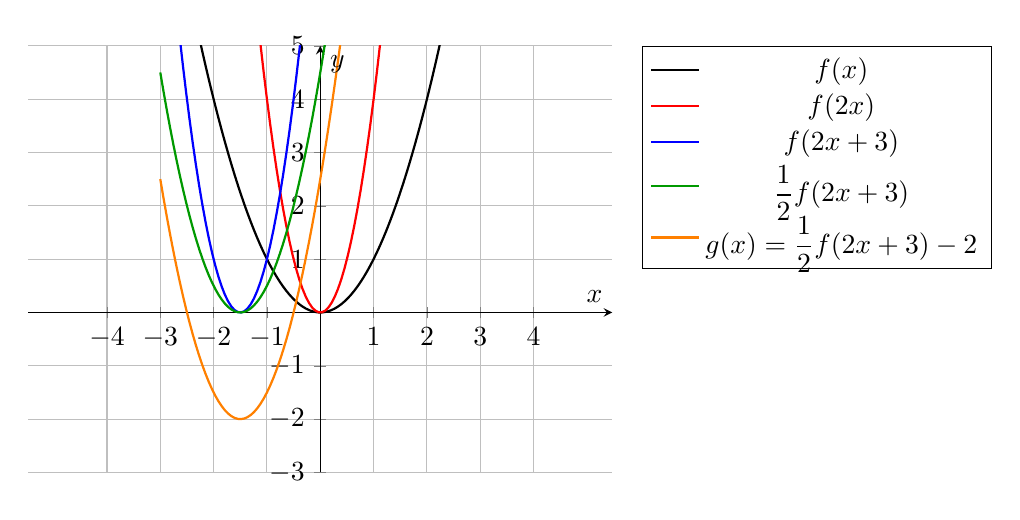
\begin{tikzpicture}
					\begin{axis}[
						axis lines=middle,
						xmin=-3, xmax=3,
						ymin=-3, ymax=5,
						xlabel={$x$},
						ylabel={$y$},
						xtick={-4,-3,-2,-1,0,1,2,3,4},
						ytick={-3,-2,-1,0,1,2,3,4,5},
						grid=both,
						width=9cm,
						height=7cm,
						axis equal,
						legend style={
							at={(1.05,1)},
							anchor=north west
						}
						]
						
						% f(x) = x^2
						\addplot[
						domain=-3:3,
						samples=100,
						thick,
						black
						] {x^2};
						\addlegendentry{$f(x)$}
						
						% Step 1: f(2x) -- horizontal compression by a factor of 2
						\addplot[
						domain=-3:3,
						samples=100,
						thick,
						red
						] {(2*x)^2};
						\addlegendentry{$f(2x)$}
						
						% Step 2: f(2x+3) -- shift left by 3/2
						\addplot[
						domain=-3:3,
						samples=100,
						thick,
						blue
						] {(2*x+3)^2};
						\addlegendentry{$f(2x+3)$}
						
						% Step 3: (1/2)f(2x+3) -- vertical compression by a factor of 2
						\addplot[
						domain=-3:3,
						samples=100,
						thick,
						green!60!black
						] {0.5*(2*x+3)^2};
						\addlegendentry{$\dfrac{1}{2}f(2x+3)$}
						
						% Step 4: (1/2)f(2x+3)-2 -- shift down 2
						\addplot[
						domain=-3:3,
						samples=100,
						thick,
						orange
						] {0.5*(2*x+3)^2-2};
						\addlegendentry{$g(x)=\dfrac{1}{2}f(2x+3)-2$}
						
					\end{axis}
				\end{tikzpicture}
			\end{itemize}
		\end{solution}
		\item Determine whether the following functions are even, odd, or neither.
		\begin{enumerate}
			\item $f(x)=\dfrac{x^2}{x-1}$
			\item $f(x)=\dfrac{x^2-1}{x}$
			\item $f(x)=\sqrt{x^2-4}$
			\item $f(x)=x^{3/2}+1$
			\item $f(x)=|2x^3-1|$
			\item $f(x)=|2x^2-1|$
		\end{enumerate}
		\begin{solution}
			\begin{itemize}
				\item[(a)] The domain of the function is $(-\infty,1)\cup(1,\infty)$. Since this is not a set that is symmetric with respect to the origin, the function is neither even, nor odd.
				\item[(b)] The domain of the function is $(-\infty,0)\cup(0,\infty)$, which is a symmetric set with respect to the origin, so we proceed with checking whether $f(-x)=f(x)$ or $f(-x)=-f(x)$, or neither. We have $$f(-x)=\dfrac{(-x)^2-1}{-x}=\dfrac{x^2-1}{-x}=-\dfrac{x^2-1}{x}=-f(x).$$ Hence, the function is odd.
				\item[(c)] The domain of the function is all $x$ such that $x^2-4\geq0$, i.e. $(\infty,-2]\cup [2,\infty)$. This is a symmetric set with respect to the origin. We have $$f(-x)=\sqrt{(-x)^2-4}=\sqrt{x^2-4}=f(x).$$
				Hence, the function is even.
				\item[(d)] The domain of this function is $[0,\infty)$, which is not a symmetric set with respect to the origin. Hence, the function is neither even, nor odd.
				\item[(e)] The domain of the function is $\mathbb{R}$, which is a symmetric set with respect to the origin. We have $$f(-x)=|2(-x)^3-1|=|-2x^3-1|,$$
				so $f(-x)\neq f(x)$ and $f(-x)\neq -f(x)$. Thus, the function is neither even, nor odd.
				\item[(f)] The domain of the function is $\mathbb{R}$, which is a symmetric set with respect to the origin. We have
				$$f(-x)=|2(-x)^2-1|=|2x^2-1|=f(x).$$
				Hence, the function is even.
			\end{itemize}
		\end{solution}
		
		\item Determine whether the following statements are true or false. Justify your reasoning.
		\begin{enumerate}
			
			\item If $g(x)=f(3x)$, then the graph of $g$ is obtained by vertically compressing the graph of $f$ by a factor of $3$.
			
			\item If $g(x)=\frac{1}{3}f(x)$, then every point on the graph of $f$ is moved one-third of the way toward the $x$-axis.
			
			\item If $g(x)=-f(-x)$, then the graph of $g$ can be obtained by reflecting the graph of $f$ about the $y$-axis and then reflecting the result about the $x$-axis.
			
			\item If $f$ is an odd function, then $-f(x)$ is also an odd function.
			
			\item The function
			$
			f(x)=\sqrt{x^2-9}
			$
			is even.
			
			\item The function
			$
			f(x)=|x^3|
			$
			is odd.
			\item If the domain of a function is not symmetric about the origin, then the function cannot be even or odd.
			
			\item The graph of
			$
			g(x)=-2f(x-3)+4
			$
			can be obtained from the graph of $f$ by shifting right $3$ units, reflecting about the $y$-axis, vertically stretching by a factor of $2$, and shifting up $4$ units.
			
		\end{enumerate}
		\begin{solution}
			\begin{itemize}
				\item[(a)] False. Replacing $x$ by $3x$ produces a horizontal compression by a factor of $3$.
					
				\item[(b)] True.	Multiplying the function by $\frac{1}{3}$ multiplies every $y$-coordinate by $\frac{1}{3}$, moving each point one-third of the way toward the $x$-axis.
					
				\item[(c)] True. Replacing $x$ by $-x$ reflects the graph across the $y$-axis, and multiplying by $-1$ reflects it across the $x$-axis.
					
				\item[(d)] True. If $f$ is odd, then $f(-x)=-f(x)$. Let $g(x)=-f(x)$. Then
					$$g(-x)=-f(-x)=-[-f(x)]=f(x)=-g(x),	$$
					so $g$ is odd.
					
				\item[(e)] True. The domain is
					$(-\infty,-3]\cup[3,\infty),$
					which is symmetric about the origin. Also,
					$$f(-x)=\sqrt{(-x)^2-9}
					=\sqrt{x^2-9}
					=f(x).$$
					Therefore, $f$ is even.
					
				\item[(f)] False. Although $x^3$ is odd, taking the absolute value changes the symmetry. We have
					$$f(-x)=|-x^3|=|x^3|=f(x).$$
					Thus, $f(x)=|x^3|$ is even, not odd.
					
				\item[(g)] True. Symmetry of the domain about the origin is a necessary condition for a function to be even or odd. Therefore, if the domain is not symmetric about the origin, the function is neither even nor odd.
					
				\item[(h)] False. The reflection should be about the $x$-axis.
					
				
			\end{itemize}
		\end{solution}
	\end{enumerate}
	
	\newpage
	
		\section{Operations with Functions}
	
	\begin{enumerate}
		\item Let $f(x)=\dfrac{x}{x-2}$ and $g(x)=\dfrac{2x}{x-1}$. Find
		\begin{enumerate}
			\item $(f-g)(-2)$
			
			\item $(f+g)(1)$
		
			\item $(f-g)(2)$
		
			\item $\dfrac{f}{g}(3)$
		
			\item $\dfrac{f}{g}(0)$
		
			\item $g\cdot g(3)$
		
			\item $f\circ g(1)$
			
			\item $f\circ g(2)$.
			\item a formula for $g \circ f(x)$
			
			\item a formula for $f \circ f (x)$
			
		\end{enumerate}
		
		\begin{solution}
			\begin{itemize}
				\item[(a)]	$(f-g)(-2)=f(-2)-g(-2)=\dfrac{-2}{-2-2}-\dfrac{2(-2)}{-2-1}=\dfrac{1}{2}-\dfrac{4}{3}=-\dfrac{5}{6}$.
				\item[(b)]	$g(x)$ is not defined for $x=1$, so $(f+g)(1)$ is undefined.
				\item[(c)] 	$f(x)$ is not defined for $x=2$, so $(f-g)(2)$ is undefined.
				\item[(d)]	$\dfrac{f}{g}(3)=\dfrac{f(3)}{g(3)}=\dfrac{\dfrac{3}{3-2}}{\dfrac{2\cdot 3}{3-1}}=\dfrac{3}{3}=1$.
				\item[(e)] 	$g(0)=0$, so $\dfrac{f}{g}(0)$ is undefined.
				\item[(f)] 	$g\cdot g(3)=g(3)\cdot g(3)=3\cdot 3=9.$
				\item[(g)] $f\circ g(1)=f(g(1))$, but $g$ is not defined at $1$, so $f\circ g(1)$ is undefined.
				\item[(h)]  $f\circ g(2)=f(g(2))=f\left(\dfrac{2\cdot 2}{2-1}\right)=f(4)=\dfrac{4}{4-2}=2$.
				\item[(i)] $g\circ f(x)=g(f(x))=g\left(\dfrac{x}{x-2}\right)=\dfrac{2\cdot\dfrac{x}{x-2}}{\dfrac{x}{x-2}-1}=\dfrac{\dfrac{2x}{x-2}}{\dfrac{2}{x-2}}\\=\dfrac{2x}{x-2}\cdot \dfrac{2}{x-2}=x$.
				\item[(j)] $f\circ f(x)=f(f(x))=f\left(\dfrac{x}{x-2}\right)=\dfrac{\dfrac{x}{x-2}}{\dfrac{x}{x-2}-2}=\dfrac{\dfrac{x}{x-2}}{\dfrac{-x+4}{x-2}}=\dfrac{x}{4-x}$.
			\end{itemize}
		\end{solution}
		
		\item Use the table to find the indicated values or state that they cannot be determined based solely on the table.
		
		\begin{center}
			\begin{tabular}{c|ccccc}
				$x$ & $-2$ & $-1$ & $0$ & $1$ & $2$ \\
				\hline
				$f(x)$& 1&$-2$ &3 &0 & $-1$ \\
				$g(x)$ & 1&0 &$-1$ &2 &$-3$ \\
			\end{tabular}
		\end{center} 
		\begin{enumerate}
			\item $(f+g)(-2),(fg)(0),\dfrac{f}{g}(1),\dfrac{g}{f}(1)$
			\item $f\circ g(-2), g\circ f(0),g\circ g(1), f\circ f(2)$
		\end{enumerate}
		
		\begin{solution}
			\begin{itemize}
				\item[(a)] $(f+g)(-2)=f(-2)+g(-2)=1+1=2,\\
				(fg)(0)=f(0)g(0)=3\cdot(-1)=-3,\\
				\dfrac{f}{g}(1)=\dfrac{f(1)}{g(1)}=\dfrac{0}{2}=0,\\
				\dfrac{g}{f}(1)$ is undefined since $f(1)=0$.
				\item[(b)] $f\circ g(-2)=f(g(-2))=f(1)=0,\\
				 g\circ f(0)=g(f(0))=g(3) \text{ cannot be determined based solely on the table,}\\
				 g\circ g(1)=g(g(1))=g(2)=-3,\\
				  f\circ f(2)=f(f(2))=f(-2)$ cannot be determined based solely on the table.
			\end{itemize}
		\end{solution}
		
		\item Using the graphs of the function \textcolor{blue}{$f$} and \textcolor{red}{$g$} below, find the following values or state they cannot be determined based on the image.
		
			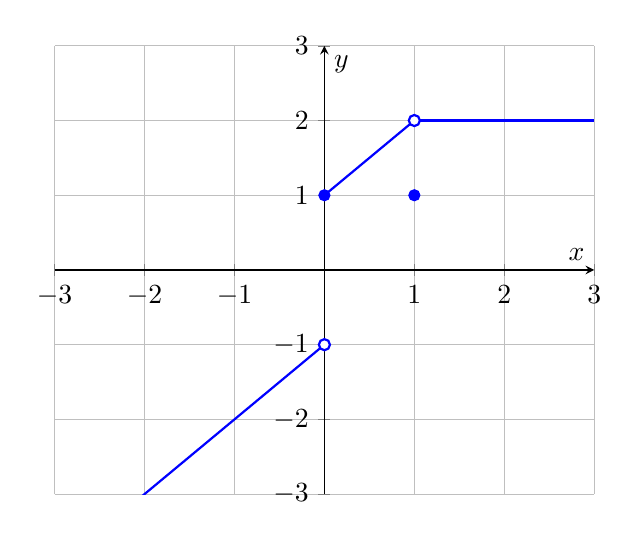
\begin{tikzpicture}
			\begin{axis}[
				axis lines = middle,
				xlabel = {$x$},
				ylabel = {$y$},
				xmin = -3, xmax = 3,
				ymin = -3, ymax = 3,
				xtick={-3,-2,-1,0,1,2,3},
				ytick={-3,-2,-1,0,1,2,3},
				grid = both
				]
				
				% y = x - 1 for x < 0
				\addplot[
				domain=-3:0,
				samples=100,
				blue,
				thick
				] {x - 1};
				
				% y = x + 1 for 0 < x < 1
				\addplot[
				domain=0:1,
				samples=100,
				blue,
				thick
				] {x + 1};
				
				% y = 2 for x > 1
				\addplot[
				domain=1:3,
				samples=100,
				blue,
				thick
				] {2};
				
				% Hole at (0,-1)
				\addplot[
				only marks,
				mark=*,
				mark size=2pt,
				fill=white,
				draw=blue,
				thick
				] coordinates {(0,-1)};
				
				% Point at (0,1)
				\addplot[
				only marks,
				mark=*,
				mark size=2pt,
				blue
				] coordinates {(0,1)};
				
				% Hole at (1,2)
				\addplot[
				only marks,
				mark=*,
				mark size=2pt,
				fill=white,
				draw=blue,
				thick
				] coordinates {(1,2)};
				
				% Point at (1,1)
				\addplot[
				only marks,
				mark=*,
				mark size=2pt,
				blue
				] coordinates {(1,1)};
				
			\end{axis}
		\end{tikzpicture}
		
		
		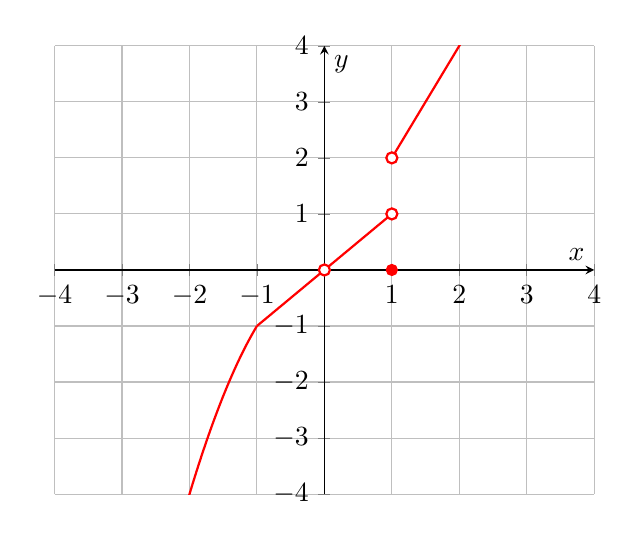
\begin{tikzpicture}
			\begin{axis}[
				axis lines = middle,
				xlabel = {$x$},
				ylabel = {$y$},
				xmin = -4, xmax = 4,
				ymin = -4, ymax = 4,
				xtick={-4,-3,-2,-1,0,1,2,3,4},
				ytick={-4,-3,-2,-1,0,1,2,3,4},
				grid = both
				]
				
				% Concave down quadratic on (-infty,-1)
				\addplot[
				domain=-3:-1,
				samples=100,
				red,
				thick
				] {-x^2};
				
				% Linear function on (-1,1)
				\addplot[
				domain=-1:1,
				samples=100,
				red,
				thick
				] {x};
				
				% Concave up quadratic y = x^2 + 1 on (1,infty)
				\addplot[
				domain=1:3,
				samples=100,
				red,
				thick
				] {2*x};
				
				% Hole at (1,2)
				\addplot[
				only marks,
				mark=*,
				mark size=2pt,
				fill=white,
				draw=red,
				thick
				] coordinates {(1,2)};
				
				% Hole at (1,1)
				\addplot[
				only marks,
				mark=*,
				mark size=2pt,
				fill=white,
				draw=red,
				thick
				] coordinates {(1,1)};
				
				% Hole at (0,0)
				\addplot[
				only marks,
				mark=*,
				mark size=2pt,
				fill=white,
				draw=red,
				thick
				] coordinates {(0,0)};
				
				% Point at (1,0)
				\addplot[
				only marks,
				mark=*,
				mark size=2pt,
				red
				] coordinates {(1,0)};
				
			\end{axis}
		\end{tikzpicture}
		
		\begin{enumerate}
			\item $(f+g)(-2),(fg)(0),\dfrac{f}{g}(1),\dfrac{g}{f}(1)$
			\item $f\circ g(-2), g\circ f(0),g\circ g(1), f\circ f(2)$
		\end{enumerate}
		
		\begin{solution}
			\begin{itemize}
				\item[(a)] $(f+g)(-2)=f(-2)+g(-2)=-3+(-4)=-7,\\
				(fg)(0) \text{ is undefined since } g(0) \text{ is undefined,}\\
				\dfrac{f}{g}(1) \text{ is undefined since } g(1)=0\\
				\dfrac{g}{f}(1)=\dfrac{g(1)}{f(1)}=\dfrac{0}{1}=0$.
				\item[(b)] $f\circ g(-2)=f(g(-2))=f(-4) \text{ cannot be determined based on the image},\\
				g\circ f(0)=g(f(0))=g(1)=0,\\
				g\circ g(1)=g(g(1))=g(0) \text{ is undefined},\\
				f\circ f(2)=f(f(2))=f(2)=2$.
			\end{itemize}
		\end{solution}
		
		\item Write the functions as a composition of at least three different functions. Note that there are several ways to do this, so the answer is not unique.
		\begin{enumerate}
			\item $f(x)=\dfrac{1}{\sqrt{x^2+1}}$
			
			\item $f(x)=3(x-1)^{3/2}$
			
			\item $f(x)=\dfrac{\sqrt{(1+2x)^3}+2\sqrt{1+2x}-1-2x}{\sqrt{1+2x}}$
		
		\end{enumerate}
		
		\begin{solution}
			\begin{itemize}
				\item[(a)] 	$f=f_1\circ f_2 \circ f_3$, where $f_1(x)=\dfrac{1}{x},f_2(x)=\sqrt{x},f_3(x)=x^2+1$
				\item[(b)] 	$f=f_1\circ f_2 \circ f_3$, where $f_1(x)=3x,f_2(x)=x^{3/2},f_3(x)=x-1$
				\item[(c)] 	$f=f_1\circ f_2 \circ f_3$, where $f_1(x)=1+2x,f_2(x)=\sqrt{x},f_3(x)=\dfrac{x^3+2x-x^2}{x}$.
			\end{itemize}
		\end{solution}
		
		\item Find the implied domain of the function $f\circ g$ and $g\circ f$, if
		\begin{enumerate}
			\item $f(x)=\sqrt{x}, g(x)=x-3$
			\item $f(x)=x+1, g(x)=\sqrt{x-2}$
			\item $f(x)=\dfrac{1}{x-2}, g(x)=x+1$
			\item $f(x)=\sqrt{x},g(x)=\dfrac{1}{x-1}$
		\end{enumerate}
		
		\begin{solution}
			\begin{itemize}
				\item[(a)] $g(x)$ is a polynomial function, so it is defined for all real numbers. We have
				$$f\circ g(x)=f(g(x))=\sqrt{x-3}.$$
				For this function to be defined, we need $x-3\geq0\iff x\geq 3$.
				
				Thus, the domain is $[3,\infty)$.
				\item[(b)] For $g(x)$ to be defined, we need $x-2\geq 0 \iff x\geq 2$. We have 
				$$f\circ g(x)=f(g(x))=\sqrt{x-2}+1,$$
				which is again defined for all $x$ such that $x\geq 2$. 
				
				Thus, the domain is $[2,\infty).$
				\item[(c)] $g(x)$ is a polynomial function, so it is defined for all real numbers. We have 
				$$f\circ g(x)
				=f(g(x))
				=\dfrac{1}{(x+1)-2}
				=\dfrac{1}{x-1},$$
				which is defined for all $x-1\neq 0 \iff x\neq 1$.
				
				Thus, the domain is $\mathbb{R}\setminus\{1\}$.
				\item[(d)] $g(x)$ is defined for all $x$ such that $x-1\neq0 \iff x\neq 1$. We have
				$$f\circ g(x)
				=f(g(x))
				=\sqrt{\frac{1}{x-1}}.$$
				which is defined for all $x\neq 1$ such that $\dfrac{1}{x-1}\geq 0$. Solving this inequality gives $x>1$.
				
				Thus, the domain is $(1,\infty).$
			\end{itemize}
		\end{solution}
		
		\item Determine whether the following statements are true or false. Justify your reasoning.
		
		\begin{enumerate}
				
			\item If $f(x)=\dfrac{x}{x-2}$ and $g(x)=\dfrac{2x}{x-1}$, then the formula for $f\circ g$ is  $f\circ g(x)=\dfrac{x}{2x-3}$.
	
			\item If $f(x)=\dfrac{x}{x-2}$, then $f(f(4))$ is undefined.
			
			\item Suppose $f(0)=2$ and $g(2)=5$. Then the value of $f\circ g(0)$ can be determined from this information.
			
			\item Suppose $f(0)=2$ and $g(2)=5$. Then the value of $g\circ f(0)$ can be determined from this information.
				
			\item If $g(0)$ is undefined, then $(fg)(0)$ must also be undefined.
			
			\item If $g(a)$ is defined and $f(g(a))$ is defined, then $f\circ g(a)$ is defined.
			
			\item If $f\circ g$ is defined at $a$, then both $f(a)$ and $g(a)$ must be defined.
			
			\item If the domain of $g$ is all real numbers and the domain of $f$ is $[0,\infty)$, then the domain of $f\circ g$ is all real numbers.
			
			\item If $f(x)=\sqrt{x}$ and $g(x)=x^2-4$, then the domain of $f\circ g$ is $(-\infty,-2]\cup[2,\infty)$.
			
			\item If $f(x)=\sqrt{x}$ and $g(x)=x^2-4$, then the domain of $g\circ f$ is	$[2,\infty)$.		
			
		\end{enumerate}
		
		\begin{solution}
			\begin{itemize}
				\item[(a)] False. $$f\circ g(x)=f(g(x))=f\left(\dfrac{2x}{x-1}\right)=\dfrac{\dfrac{2x}{x-1}}{\dfrac{2x}{x-1}-2}=\dfrac{\dfrac{2x}{x-1}}{\dfrac{2x-2(x-1)}{x-1}}=\dfrac{\dfrac{2x}{x-1}}{\dfrac{2}{x-1}}=x.$$
				\item[(b)] True. $f(4)=\dfrac{4}{4-2}=2$ and $f(x)$ is undefined at 2.
				\item[(c)] False. $f\circ g (0)=f(g(0))$ but there is no information given about the value of $g(0)$.
				\item[(d)] True. $g\circ f(0)=g(f(0))=g(2)=5$.
				\item[(e)] True. In order for $(fg)(0)$ to be defined, both $f(0)$ and $g(0)$ have to be defined.
				\item[(f)] True. $f\circ g(a)=f(g(a))$, so this follows by definition.
				\item[(g)] False. If $f\circ g$ is defined at $a$, then $g(a)$ and $f(g(a))$ must be defined. However, $f(a)$ can be undefined. For example, let $f(x)=\sqrt{x},g(x)=x+1$. Then
				$f\circ g(-1)=f(0)=0$
				is defined, even though $f(-1)$ is undefined.
				\item[(h)] False. The domain of $f\circ g$ consists of all $x$ such that $g(x)\geq 0$. This is not necessarily all real numbers.
				\item[(i)] True. $g(x)$ is a polynomial function so it is defined for all real numbers. We have 
				$$f\circ g(x)=f(g(x))=f(x^2-4)=\sqrt{x^2-4}.$$
				The domain of this function consists of all $x$ such that $x^2-4\geq 0$, i.e., all $x$ such that $x\leq -2$ or $x\geq 2$. Thus, the domain is $(-\infty,-2]\cup[2,\infty)$.
				\item[(j)] False. We have $g\circ f(x)=g(f(x))
				=g(\sqrt{x})=(\sqrt{x})^2-4=x-4$.
				Since $f(x)=\sqrt{x}$, we need $x\geq0$.
				The function $g$ is defined for all real numbers, so there are no additional restrictions. Thus, the domain is $[0,\infty)$.
			\end{itemize}
		\end{solution}
		
	\end{enumerate}
	
	\newpage
	\section{Solving Inequalities}
	
	\begin{enumerate}
		\item Find all the real values of $x$ that satisfy the following inequalities. Write your answer using interval notation or set builder notation.
		\begin{enumerate}
			\item $5x-3>2x+1$
			
			\item $(x-2)^2\leq (x+1)^2$
			
			\item $x^2-4x+3\leq 0$
			
			
			\item $x(x-1)>(x-\dfrac{1}{2})^2$
			
			\item $3x^2+5x+7>0$
			
			\item $3x^2+5x+7\leq 0$
			
			\item $\dfrac{2x-1}{x+2}\geq 0$
			
			\item $\dfrac{2x-1}{x+2} \geq 2$
			
			\item $(x+1)(2x-1)^2(2-x)<0$
			
			
			\item $\dfrac{(x+1)(2x-1)^2}{2-x}\leq 0$
			
			\item $\dfrac{x^2+8x+7}{x-1}>2$
		\end{enumerate}
		
		\begin{solution}
			\begin{itemize}
				\item[(a)] \begin{align*}
					5x-3&>3x+1\\
					5x-2x&>1+3\\
					3x&>4\\
					x&>\dfrac{4}{3}
				\end{align*} 
				The solution is $\left(\dfrac{4}{3},\infty\right)$.
				\item[(b)] 		\begin{align*}
					(x-2)^2&\leq (x+1)^2\\
					x^2-4x+3 &\leq x^2+2x+1\\
					-4x-2x&\leq 1-4\\
					-6x &\leq -3\\
					x &\geq \dfrac{1}{2}
				\end{align*}
				
				The solution is $\left[\dfrac{1}{2},\infty\right]$.
				\item[(c)] 	We need to solve the inequality $x^2-4x+3\leq 0$. In other words, we need to find all $x$ such that $g(x) \geq 0$, where $g(x)=x^2-4x+3$. The first step is to find the domain of $g(x)$. The domain of $g(x)$ is $\mathbb{R}$. Next, we find the zeroes by solving the equation $g(x)=0$.
				
				\begin{align*}
					x^2-4x+3&=0\\
					(x-1)(x-3)&=0\\
					x=1 \text{ or } x&=3.
				\end{align*}
				
				Both $1$ and $3$ are in the domain of $g(x)$, so they are both zeroes. Using this information, we can draw a sign chart. 
				
				\[
				\begin{tikzpicture}[scale=1]
					\draw[->] (-5,0) -- (5,0);
					
					\draw (-2.5,0) node[circle,blue,fill,inner sep=2pt]{};
					\draw (1.5,0) node[circle,blue,fill,inner sep=2pt]{};
					%	\draw[blue, thick, fill=white] (0,0) circle (2.5pt);
					
					\node at (-2.5, .5) {1};
					\node at (1.5, .5) {3};
					%\node at (0, .5) {$0$};
					\node at (-5,.5) {$g\colon$};
					\node at (-3.5,.5) {$+$};
					\node at (-0.4,.5) {$-$};
					\node at (3, .5) {$+$};
				\end{tikzpicture}
				\]
				
				Since we are trying to find all $x$ such that $x^2-4x+3$ is negative or equal to $0$, using the sign chart, the solution is $[1.3]$.
				\item[(d)] 	\begin{align*}
					x(x-1)&>(x-1\dfrac{1}{2})^2\\
					x^2-x&>x^2-x+\dfrac{1}{4}\\
					0&>\dfrac{1}{4}.
				\end{align*}
				
				Since $0>\dfrac{1}{4}$ is false for any $x$, there is no real solution to this inequality. We say that the solution is $\emptyset$ (the \textit{empty set}).
				\item[(e)] 	We need to solve the inequality $3x^2+5x+7> 0$. In other words, we need to find all $x$ such that $g(x) \geq 0$, where $g(x)=3x^2+5x+7$. However, this equation has no real solutions, so $g(x)$ is either positive everywhere or negative everywhere. We notice that for all $x$, $g(x)>0$. Hence, all real numbers satisfy this inequality, so the solution is $(-\infty,\infty)=\mathbb{R}$.
				\item[(f)] 	From the previous exercise, we notice there are no $x$ such that $3x^2+5x+7\leq 0$, so the solution is $\emptyset$.
				\item[(g)] 	We need to solve the inequality $\dfrac{2x-1}{x+2}\geq 0$. In other words, we need to find all $x$ such that $g(x) \geq 0$, where $g(x)=\dfrac{2x-1}{x+2}$. The first step is to find the domain of $g(x)$, which is all real numbers such that $x+2\neq0$. Thus, the domain of $g(x)$ is $(-\infty, -2) \cup (-2, \infty) $. Next, we find the zeroes by solving the equation $g(x)=0$.
				
				\begin{align*}
					\dfrac{2x-1}{x+2}&=0\\
					2x-1&=0\\
					x&=\dfrac{1}{2}.
				\end{align*}
				
				$\dfrac{1}{2}$ is in the domain of $g(x)$, so it is a zero. Using this information, we can draw a sign chart. 
				
				\[
				\begin{tikzpicture}[scale=1]
					\draw[->] (-5,0) -- (5,0);
					
					%\draw (-2.5,0) node[circle,blue,fill,inner sep=2pt]{};
					\draw (1.5,0) node[circle,blue,fill,inner sep=2pt]{};
					\draw[blue, thick, fill=white] (-2.5,0) circle (2.5pt);
					
					\node at (-2.5, .5) {-2};
					\node at (1.5, .5) {1/2};
					%\node at (0, .5) {$0$};
					\node at (-5,.5) {$g\colon$};
					\node at (-3.5,.5) {$+$};
					\node at (-0.4,.5) {$-$};
					\node at (3, .5) {$+$};
				\end{tikzpicture}
				\]		
				
				Since we are trying to find all $x$ such that $\dfrac{2x-1}{x+2}$ is positive or equal to $0$, using the sign chart, we conclude that the solution is $(\infty, -2) \cup [1/2, \infty]$.
				\item[(h)] 		\begin{align*}
					\dfrac{2x-1}{x+2}&\geq 2\\
					\dfrac{2x-1}{x+2} - 2&\geq 0\\
					\dfrac{2x-1-2x-4}{x+2} &\geq 0\\
					\dfrac{-5}{x+2}&\geq 0
				\end{align*}
				
				We need to solve the inequality $\dfrac{-5}{x+2}\geq 0$. In other words, we need to find all $x$ such that $g(x) \geq 0$, where $g(x)=\dfrac{-5}{x+2}$. The first step is to find the domain of $g(x)$. The domain of $g(x)$ is $(-\infty, -2) \cup (-2, \infty) $. Next, we find the zeroes by solving the equation $g(x)=0$.
				\begin{align*}
					\dfrac{-5}{x+2}&=0\\
					-5&=0
				\end{align*}
				
				so this equation has no solutions, and hence $g(x)$ has no zeroes. This does NOT mean we cannot solve the inequality. 
				
				We can still draw a sign chart. 
				
				\[
				\begin{tikzpicture}[scale=1]
					\draw[->] (-4,0) -- (0,0);
					
					%\draw (-2.5,0) node[circle,blue,fill,inner sep=2pt]{};
					%\draw (1.5,0) node[circle,blue,fill,inner sep=2pt]{};
					\draw[blue, thick, fill=white] (-2,0) circle (2.5pt);
					
					\node at (-2, .5) {-2};
					%	\node at (1.5, .5) {1/2};
					%\node at (0, .5) {$0$};
					\node at (-5,.5) {$g\colon$};
					\node at (-3.5,.5) {$+$};
					\node at (-0.5,.5) {$-$};
					%	\node at (3, .5) {$+$};
				\end{tikzpicture}
				\]		
				
				Since we are trying to find all $x$ such that $\dfrac{-5}{x+2}$ is positive or equal to $0$, using the sign chart, we conclude that the solution is $(-\infty,-2)$.
				\item[(i)] 		We need to solve the inequality $(x+1)(2x-1)^2(2-x)< 0$. In other words, we need to find all $x$ such that $g(x) < 0$, where $g(x)=(x+1)(2x-1)^2(2-x)$. The first step is to find the domain of $g(x)$. The domain of $g(x)$ is $\mathbb{R}$. Next, we find the zeroes by solving the equation $(x+1)(2x-1)^2(2-x)=0$. The solutions are $x=-1,x=\dfrac{1}{2},x=2$ and all three solutions are in the domain.
				We draw a sign chart. 
				
				\[
				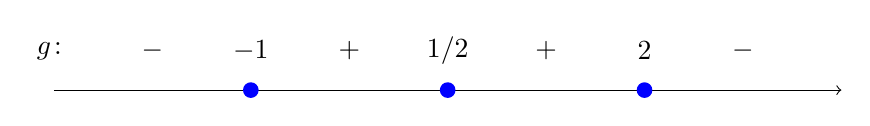
\begin{tikzpicture}[scale=1]
					\draw[->] (-7,0) -- (3,0);
					
					\draw (-2,0) node[circle,blue,fill,inner sep=2pt]{};
					\draw (-4.5,0) node[circle,blue,fill,inner sep=2pt]{};
					\draw (0.5,0) node[circle,blue,fill,inner sep=2pt]{};
					%\draw[blue, thick, fill=white] (-2,0) circle (2.5pt);
					
					\node at (-2, .5) {1/2};
					\node at (-4.5, .5) {$-1$};
					\node at (0.5, .5) {2};
					\node at (-7,.5) {$g\colon$};
					\node at (-3.25,.5) {$+$};
					\node at (-0.75,.5) {$+$};
					\node at (1.75, .5) {$-$};
					\node at (-5.75, .5) {$-$};
				\end{tikzpicture}
				\]		
				
				Since we are trying to find all $x$ such that $(x+1)(2x-1)^2(2-x)$ is negative, using the sign chart, we conclude that the solution is $(-\infty,-1)\cup (2,\infty)$.
				\item[(j)] 	We need to solve the inequality $\dfrac{(x+1)(2x-1)^2}{2-x}\leq 0$. In other words, we need to find all $x$ such that $g(x) \leq 0$, where $g(x)=\dfrac{(x+1)(2x-1)^2}{2-x}$. The first step is to find the domain of $g(x)$. The domain of $g(x)$ is $\mathbb{R}\setminus \{2\}$. Next, we find the zeroes by solving the equation $\dfrac{(x+1)(2x-1)^2}{2-x}=0$. The solutions are $x=-1,x=\dfrac{1}{2}$ and both are in the domain.
				We draw a sign chart. 
				
				\[
				\begin{tikzpicture}[scale=1]
					\draw[->] (-7,0) -- (3,0);
					
					\draw (-2,0) node[circle,blue,fill,inner sep=2pt]{};
					\draw (-4.5,0) node[circle,blue,fill,inner sep=2pt]{};
					%\draw (0.5,0) node[circle,blue,fill,inner sep=2pt]{};
					\draw[blue, thick, fill=white] (0.5,0) circle (2.5pt);
					
					\node at (-2, .5) {1/2};
					\node at (-4.5, .5) {$-1$};
					\node at (0.5, .5) {2};
					\node at (-7,.5) {$g\colon$};
					\node at (-3.25,.5) {$+$};
					\node at (-0.75,.5) {$+$};
					\node at (1.75, .5) {$-$};
					\node at (-5.75, .5) {$-$};
				\end{tikzpicture}
				\]		
				
				Since we are trying to find all $x$ such that $\dfrac{(x+1)(2x-1)^2}{2-x}\leq 0$ is negative or 0, using the sign chart, we conclude that the solution is $(-\infty,-1]\cup (2,\infty)$.
				\item[(k)] 	\begin{align*}
					\dfrac{x^2+8x+7}{x-1}>2 &\iff \dfrac{x^2+8x+7}{x-1}-2>0\\
					&\iff \dfrac{x^2+8x+7}{x-1}-\dfrac{2x-2}{x-1}>0\\
					&\iff \dfrac{x^2+6x+9}{x-1}>0\\
					&\iff \dfrac{(x+3)^2}{x-1}>0					
				\end{align*}
				
				We can use a sign chart as previously to solve the inequality. However, notice that $(x+3)^2\geq 0$ for all $x\in\mathbb{R}$, so we only need to find the $x$ such that $x-1>0$ i.e., $x>1$. Thus, the solution is $(1,\infty)$.
			\end{itemize}
		\end{solution}
		\newpage
		\item Determine whether the following statements are true or false. Justify your reasoning.
		
		\begin{enumerate}
			\item If $a,b\in \mathbb{R}$ are such that $a\leq b$, then $a^2\leq ab$.
		
			\item If $a,b\in \mathbb{R}$ are such that $a\leq b$, then $a^3\leq 2a^2$.
		
			\item If $a,b\in \mathbb{R}$ are such that $a< b$, then $a^3< a^2b$.
		
			\item If $a,b\in \mathbb{R}\setminus\{0\}$ are such that $a< b$, then $\dfrac{1}{a}>\dfrac{1}{b}$.
		
			\item If $a,b\in \mathbb{R}$ are such that $0<a< b$, then $\dfrac{1}{a}>\dfrac{1}{b}$.
			
			\end{enumerate}
			
			\begin{solution}
				\begin{itemize}
					\item[(a)] False. Multiplying both sides of an inequality by a negative number changes the sign. For example, take $a=-1,b=1$. Then $a=-1\leq 1=b$, but $a^2=1>-1=ab$.
					\item[(b)] True. $a^2$ is either positive or $0$. If $a^2>0$, multiplying both sides of the inequality by $a^2$ will not change the sign. If $a^2=0$, i.e. $a=0$, then we get $a^3=0\leq0=2a^2$ which is also true.
					\item[(c)] 	False. If $a=0, b=1$, it is not true that $a^3=0 < 0=a^2b$.
					\item[(d)] False. If $a=-1, b=1$, it is not true that $\dfrac{1}{a}=-1 > 1=\dfrac{1}{b}$
					\item[(e)] 	True. If we multiply both sides of the inequality by $ab>0$, then we get a true statement $b>a$.
				\end{itemize}
			\end{solution}
			\end{enumerate}
			
			
		

\end{document}
